% Options for packages loaded elsewhere
\PassOptionsToPackage{unicode}{hyperref}
\PassOptionsToPackage{hyphens}{url}
%
\documentclass[
]{article}
\usepackage{amsmath,amssymb}
\usepackage{iftex}
\ifPDFTeX
  \usepackage[T1]{fontenc}
  \usepackage[utf8]{inputenc}
  \usepackage{textcomp} % provide euro and other symbols
\else % if luatex or xetex
  \usepackage{unicode-math} % this also loads fontspec
  \defaultfontfeatures{Scale=MatchLowercase}
  \defaultfontfeatures[\rmfamily]{Ligatures=TeX,Scale=1}
\fi
\usepackage{lmodern}
\ifPDFTeX\else
  % xetex/luatex font selection
\fi
% Use upquote if available, for straight quotes in verbatim environments
\IfFileExists{upquote.sty}{\usepackage{upquote}}{}
\IfFileExists{microtype.sty}{% use microtype if available
  \usepackage[]{microtype}
  \UseMicrotypeSet[protrusion]{basicmath} % disable protrusion for tt fonts
}{}
\makeatletter
\@ifundefined{KOMAClassName}{% if non-KOMA class
  \IfFileExists{parskip.sty}{%
    \usepackage{parskip}
  }{% else
    \setlength{\parindent}{0pt}
    \setlength{\parskip}{6pt plus 2pt minus 1pt}}
}{% if KOMA class
  \KOMAoptions{parskip=half}}
\makeatother
\usepackage{xcolor}
\usepackage[margin=1in]{geometry}
\usepackage{color}
\usepackage{fancyvrb}
\newcommand{\VerbBar}{|}
\newcommand{\VERB}{\Verb[commandchars=\\\{\}]}
\DefineVerbatimEnvironment{Highlighting}{Verbatim}{commandchars=\\\{\}}
% Add ',fontsize=\small' for more characters per line
\usepackage{framed}
\definecolor{shadecolor}{RGB}{248,248,248}
\newenvironment{Shaded}{\begin{snugshade}}{\end{snugshade}}
\newcommand{\AlertTok}[1]{\textcolor[rgb]{0.94,0.16,0.16}{#1}}
\newcommand{\AnnotationTok}[1]{\textcolor[rgb]{0.56,0.35,0.01}{\textbf{\textit{#1}}}}
\newcommand{\AttributeTok}[1]{\textcolor[rgb]{0.13,0.29,0.53}{#1}}
\newcommand{\BaseNTok}[1]{\textcolor[rgb]{0.00,0.00,0.81}{#1}}
\newcommand{\BuiltInTok}[1]{#1}
\newcommand{\CharTok}[1]{\textcolor[rgb]{0.31,0.60,0.02}{#1}}
\newcommand{\CommentTok}[1]{\textcolor[rgb]{0.56,0.35,0.01}{\textit{#1}}}
\newcommand{\CommentVarTok}[1]{\textcolor[rgb]{0.56,0.35,0.01}{\textbf{\textit{#1}}}}
\newcommand{\ConstantTok}[1]{\textcolor[rgb]{0.56,0.35,0.01}{#1}}
\newcommand{\ControlFlowTok}[1]{\textcolor[rgb]{0.13,0.29,0.53}{\textbf{#1}}}
\newcommand{\DataTypeTok}[1]{\textcolor[rgb]{0.13,0.29,0.53}{#1}}
\newcommand{\DecValTok}[1]{\textcolor[rgb]{0.00,0.00,0.81}{#1}}
\newcommand{\DocumentationTok}[1]{\textcolor[rgb]{0.56,0.35,0.01}{\textbf{\textit{#1}}}}
\newcommand{\ErrorTok}[1]{\textcolor[rgb]{0.64,0.00,0.00}{\textbf{#1}}}
\newcommand{\ExtensionTok}[1]{#1}
\newcommand{\FloatTok}[1]{\textcolor[rgb]{0.00,0.00,0.81}{#1}}
\newcommand{\FunctionTok}[1]{\textcolor[rgb]{0.13,0.29,0.53}{\textbf{#1}}}
\newcommand{\ImportTok}[1]{#1}
\newcommand{\InformationTok}[1]{\textcolor[rgb]{0.56,0.35,0.01}{\textbf{\textit{#1}}}}
\newcommand{\KeywordTok}[1]{\textcolor[rgb]{0.13,0.29,0.53}{\textbf{#1}}}
\newcommand{\NormalTok}[1]{#1}
\newcommand{\OperatorTok}[1]{\textcolor[rgb]{0.81,0.36,0.00}{\textbf{#1}}}
\newcommand{\OtherTok}[1]{\textcolor[rgb]{0.56,0.35,0.01}{#1}}
\newcommand{\PreprocessorTok}[1]{\textcolor[rgb]{0.56,0.35,0.01}{\textit{#1}}}
\newcommand{\RegionMarkerTok}[1]{#1}
\newcommand{\SpecialCharTok}[1]{\textcolor[rgb]{0.81,0.36,0.00}{\textbf{#1}}}
\newcommand{\SpecialStringTok}[1]{\textcolor[rgb]{0.31,0.60,0.02}{#1}}
\newcommand{\StringTok}[1]{\textcolor[rgb]{0.31,0.60,0.02}{#1}}
\newcommand{\VariableTok}[1]{\textcolor[rgb]{0.00,0.00,0.00}{#1}}
\newcommand{\VerbatimStringTok}[1]{\textcolor[rgb]{0.31,0.60,0.02}{#1}}
\newcommand{\WarningTok}[1]{\textcolor[rgb]{0.56,0.35,0.01}{\textbf{\textit{#1}}}}
\usepackage{graphicx}
\makeatletter
\def\maxwidth{\ifdim\Gin@nat@width>\linewidth\linewidth\else\Gin@nat@width\fi}
\def\maxheight{\ifdim\Gin@nat@height>\textheight\textheight\else\Gin@nat@height\fi}
\makeatother
% Scale images if necessary, so that they will not overflow the page
% margins by default, and it is still possible to overwrite the defaults
% using explicit options in \includegraphics[width, height, ...]{}
\setkeys{Gin}{width=\maxwidth,height=\maxheight,keepaspectratio}
% Set default figure placement to htbp
\makeatletter
\def\fps@figure{htbp}
\makeatother
\setlength{\emergencystretch}{3em} % prevent overfull lines
\providecommand{\tightlist}{%
  \setlength{\itemsep}{0pt}\setlength{\parskip}{0pt}}
\setcounter{secnumdepth}{-\maxdimen} % remove section numbering
\ifLuaTeX
  \usepackage{selnolig}  % disable illegal ligatures
\fi
\IfFileExists{bookmark.sty}{\usepackage{bookmark}}{\usepackage{hyperref}}
\IfFileExists{xurl.sty}{\usepackage{xurl}}{} % add URL line breaks if available
\urlstyle{same}
\hypersetup{
  pdftitle={Taller 1},
  hidelinks,
  pdfcreator={LaTeX via pandoc}}

\title{Taller 1}
\author{}
\date{\vspace{-2.5em}2024-02-07}

\begin{document}
\maketitle

\begin{verbatim}
## Warning: package 'gridExtra' was built under R version 4.3.2
\end{verbatim}

\begin{verbatim}
## Warning: package 'rvest' was built under R version 4.3.2
\end{verbatim}

\begin{verbatim}
## Warning: package 'tidyverse' was built under R version 4.3.2
\end{verbatim}

\begin{verbatim}
## Warning: package 'ggplot2' was built under R version 4.3.2
\end{verbatim}

\begin{verbatim}
## Warning: package 'tidyr' was built under R version 4.3.2
\end{verbatim}

\begin{verbatim}
## Warning: package 'purrr' was built under R version 4.3.2
\end{verbatim}

\begin{verbatim}
## Warning: package 'forcats' was built under R version 4.3.2
\end{verbatim}

\begin{verbatim}
## Warning: package 'lubridate' was built under R version 4.3.2
\end{verbatim}

\begin{verbatim}
## -- Attaching core tidyverse packages ------------------------ tidyverse 2.0.0 --
## v dplyr     1.1.3     v readr     2.1.4
## v forcats   1.0.0     v stringr   1.5.0
## v ggplot2   3.4.4     v tibble    3.2.1
## v lubridate 1.9.3     v tidyr     1.3.1
## v purrr     1.0.2     
## -- Conflicts ------------------------------------------ tidyverse_conflicts() --
## x dplyr::combine()        masks gridExtra::combine()
## x dplyr::filter()         masks stats::filter()
## x readr::guess_encoding() masks rvest::guess_encoding()
## x dplyr::lag()            masks stats::lag()
## i Use the conflicted package (<http://conflicted.r-lib.org/>) to force all conflicts to become errors
\end{verbatim}

\begin{verbatim}
## Warning: package 'zoo' was built under R version 4.3.2
\end{verbatim}

\begin{verbatim}
## 
## Attaching package: 'zoo'
## 
## The following objects are masked from 'package:base':
## 
##     as.Date, as.Date.numeric
\end{verbatim}

\begin{verbatim}
## Warning: package 'ggthemes' was built under R version 4.3.2
\end{verbatim}

\begin{verbatim}
## Warning: package 'caTools' was built under R version 4.3.2
\end{verbatim}

\begin{verbatim}
## Warning: package 'broom' was built under R version 4.3.2
\end{verbatim}

\begin{verbatim}
## Warning: package 'pacman' was built under R version 4.3.2
\end{verbatim}

\begin{verbatim}
## Installing package into 'C:/Users/HP-Laptop/AppData/Local/R/win-library/4.3'
## (as 'lib' is unspecified)
## also installing the dependencies 'R.oo', 'R.methodsS3', 'writexl', 'R.utils'
\end{verbatim}

\begin{verbatim}
## Warning: unable to access index for repository http://www.stats.ox.ac.uk/pub/RWin/bin/windows/contrib/4.3:
##   no fue posible abrir la URL 'http://www.stats.ox.ac.uk/pub/RWin/bin/windows/contrib/4.3/PACKAGES'
\end{verbatim}

\begin{verbatim}
## package 'R.oo' successfully unpacked and MD5 sums checked
## package 'R.methodsS3' successfully unpacked and MD5 sums checked
## package 'writexl' successfully unpacked and MD5 sums checked
## package 'R.utils' successfully unpacked and MD5 sums checked
## package 'rio' successfully unpacked and MD5 sums checked
## 
## The downloaded binary packages are in
##  C:\Users\HP-Laptop\AppData\Local\Temp\RtmpSmc3SV\downloaded_packages
\end{verbatim}

\begin{verbatim}
## 
## rio installed
\end{verbatim}

\begin{verbatim}
## Warning: package 'rio' was built under R version 4.3.2
\end{verbatim}

\begin{verbatim}
## Installing package into 'C:/Users/HP-Laptop/AppData/Local/R/win-library/4.3'
## (as 'lib' is unspecified)
## also installing the dependencies 'listenv', 'parallelly', 'future', 'globals', 'shape', 'future.apply', 'numDeriv', 'progressr', 'SQUAREM', 'diagram', 'lava', 'prodlim', 'proxy', 'iterators', 'clock', 'gower', 'hardhat', 'ipred', 'timeDate', 'e1071', 'foreach', 'ModelMetrics', 'plyr', 'pROC', 'recipes', 'reshape2'
\end{verbatim}

\begin{verbatim}
## Warning: unable to access index for repository http://www.stats.ox.ac.uk/pub/RWin/bin/windows/contrib/4.3:
##   no fue posible abrir la URL 'http://www.stats.ox.ac.uk/pub/RWin/bin/windows/contrib/4.3/PACKAGES'
\end{verbatim}

\begin{verbatim}
## package 'listenv' successfully unpacked and MD5 sums checked
## package 'parallelly' successfully unpacked and MD5 sums checked
## package 'future' successfully unpacked and MD5 sums checked
## package 'globals' successfully unpacked and MD5 sums checked
## package 'shape' successfully unpacked and MD5 sums checked
## package 'future.apply' successfully unpacked and MD5 sums checked
## package 'numDeriv' successfully unpacked and MD5 sums checked
## package 'progressr' successfully unpacked and MD5 sums checked
## package 'SQUAREM' successfully unpacked and MD5 sums checked
## package 'diagram' successfully unpacked and MD5 sums checked
## package 'lava' successfully unpacked and MD5 sums checked
## package 'prodlim' successfully unpacked and MD5 sums checked
## package 'proxy' successfully unpacked and MD5 sums checked
## package 'iterators' successfully unpacked and MD5 sums checked
## package 'clock' successfully unpacked and MD5 sums checked
## package 'gower' successfully unpacked and MD5 sums checked
## package 'hardhat' successfully unpacked and MD5 sums checked
## package 'ipred' successfully unpacked and MD5 sums checked
## package 'timeDate' successfully unpacked and MD5 sums checked
## package 'e1071' successfully unpacked and MD5 sums checked
## package 'foreach' successfully unpacked and MD5 sums checked
## package 'ModelMetrics' successfully unpacked and MD5 sums checked
## package 'plyr' successfully unpacked and MD5 sums checked
## package 'pROC' successfully unpacked and MD5 sums checked
## package 'recipes' successfully unpacked and MD5 sums checked
## package 'reshape2' successfully unpacked and MD5 sums checked
## package 'caret' successfully unpacked and MD5 sums checked
## 
## The downloaded binary packages are in
##  C:\Users\HP-Laptop\AppData\Local\Temp\RtmpSmc3SV\downloaded_packages
\end{verbatim}

\begin{verbatim}
## 
## caret installed
\end{verbatim}

\begin{verbatim}
## Warning: package 'caret' was built under R version 4.3.2
\end{verbatim}

\begin{verbatim}
## Installing package into 'C:/Users/HP-Laptop/AppData/Local/R/win-library/4.3'
## (as 'lib' is unspecified)
## also installing the dependency 'repr'
\end{verbatim}

\begin{verbatim}
## Warning: unable to access index for repository http://www.stats.ox.ac.uk/pub/RWin/bin/windows/contrib/4.3:
##   no fue posible abrir la URL 'http://www.stats.ox.ac.uk/pub/RWin/bin/windows/contrib/4.3/PACKAGES'
\end{verbatim}

\begin{verbatim}
## package 'repr' successfully unpacked and MD5 sums checked
## package 'skimr' successfully unpacked and MD5 sums checked
## 
## The downloaded binary packages are in
##  C:\Users\HP-Laptop\AppData\Local\Temp\RtmpSmc3SV\downloaded_packages
\end{verbatim}

\begin{verbatim}
## 
## skimr installed
\end{verbatim}

\begin{verbatim}
## Warning: package 'skimr' was built under R version 4.3.2
\end{verbatim}

\begin{Shaded}
\begin{Highlighting}[]
\ControlFlowTok{if}\NormalTok{ (}\SpecialCharTok{!}\FunctionTok{requireNamespace}\NormalTok{(}\StringTok{"zoo"}\NormalTok{, }\AttributeTok{quietly =} \ConstantTok{TRUE}\NormalTok{)) \{}
  \FunctionTok{install.packages}\NormalTok{(}\StringTok{"zoo"}\NormalTok{)\}}
\end{Highlighting}
\end{Shaded}

\hypertarget{introduccion}{%
\section{1. Introduccion}\label{introduccion}}

El objetivo de este informe es encontrar los determinantes del salario
de las personas encuestadas en Bogotá y realizar una predicción del
mismo. Encontrar los determinantes del salario es importante porque
proporciona una guía tanto en términos personales como de política
económica cuando se busca aumentar los ingresos de las personas. Desde
la perspectiva de la política económica, aumentar los ingresos reales de
las personas puede contribuir al mejoramiento de su calidad de vida. Por
lo tanto, si se conocen los factores que pueden aumentar su capacidad
adquisitiva, es importante desarrollar políticas públicas orientadas en
ese sentido. Por otro lado, el estudio de los determinantes del salario
también es útil para las personas que ya tienen un empleo y aspiran a
mejorar sus condiciones de vida. Si se encuentra, por ejemplo, que la
educación es clave, es en este ámbito donde el trabajador debe centrar
sus esfuerzos para mejorar.

Desde la teoría económica, la ecuación de Mincer es un punto de partida
para estudiar los determinantes del salario laboral. Este modelo estima
el impacto de un año adicional de estudios en las rentas laborales de
los individuos (Mincer, 1974). La ecuación tradicional de Mincer se
puede estimar mediante mínimos cuadrados ordinarios (MCO), utilizando
como variable dependiente los ingresos y como variables independientes
los años de educación, la experiencia laboral y el cuadrado de esta
última.

\[ln(w) = \beta_{0} + \beta_{1}S + \beta_{2}Exp + \beta_{3}Exp^2 + \epsilon\]
Donde: - \(w\) son los ingresos del individuo. - \(S\) es el número de
años de educación formal completada. - \(\text{Exp}\) son los años de
experiencia laboral. - \(\epsilon\) es el término de perturbación
aleatoria que se distribuye según una Normal
\(\mathcal{N}(0, \sigma_{\epsilon}^2)\).

Para este estudio, se utilizará información de la Gran Encuesta
Integrada de Hogares (GEIH). Esta encuesta solicita información sobre
las condiciones de empleo de las personas y las características
generales de la población. Por lo tanto, tenemos los insumos necesarios
para encontrar los determinantes del salario.

Con base en lo anterior, podemos iniciar el análisis de las siguientes
variables:

\begin{itemize}
\tightlist
\item
  Edad (Age)
\item
  Cuenta propia (Self-employed)
\item
  Estrato (Socioeconomic stratum)
\item
  Formal (Formal employment)
\item
  Horas trabajadas la semana pasada (Actualhours worked previous week)
\item
  Horas trabajadas habitualmente (Usual weeklyhours worked)
\item
  Informal (Informal employment)
\item
  Ingreso total (Totalincome)
\item
  Educación (Max. Education level attained)
\item
  Oficio (Occupation)
\item
  Experiencia (Experience)
\item
  Salario (Salary)
\item
  Sexo (Sex)
\item
  Horas trabajadas(Total hours worked)
\item
  Tamaño de la empresa (Company size)
\end{itemize}

\hypertarget{datos}{%
\section{2. Datos}\label{datos}}

\hypertarget{lectura-de-los-datos}{%
\subsection{Lectura de los datos}\label{lectura-de-los-datos}}

El proceso para leer los datos consiste en hacer un web scraping a la
información que se encuentra en esta página web:
\url{https://ignaciomsarmiento.github.io/GEIH2018sample/.} Los datos
están particionados en 10 páginas diferentes, por lo cual se tiene que
hacer un proceso iterativo. En primer lugar, se guarda en la variable
\textbf{\texttt{url\_base}} la dirección web de la que se debe extraer
la información. Hay un ligero cambio respecto a la URL general y este es
que las tablas se encuentran un poco más anidadas, por lo que se debe
completar la URL. Como la base de datos completa se encuentra separada
en 10 partes, el proceso se debe repetir el mismo número de veces.
Primero se crea una lista vacía llamada \textbf{\texttt{tables\_list}},
en esta lista se guarda la información extraída de la página en cada
iteración. Dentro del bucle \textbf{\texttt{for}}, se va modificando la
ruta de extracción para que haga un recorrido por todas las direcciones
donde se encuentran los datos. Esto es relativamente sencillo debido a
que lo único que cambia es el número de la página; por esto, el iterador
es un entero.

Cuando se hace el proceso iterativo en las 10 páginas, estas quedan
anidadas en la lista vacía \textbf{\texttt{tables\_list}}. Para darle un
formato manejable en el proceso de machine learning, se concatenan en
una sola sabana de datos con formato \textbf{\texttt{tibble}}. Como la
cantidad de datos es considerable, este proceso dura aproximadamente 8
minutos.

\begin{Shaded}
\begin{Highlighting}[]
\NormalTok{t1}\OtherTok{\textless{}{-}}\FunctionTok{Sys.time}\NormalTok{()}

\NormalTok{url\_base}\OtherTok{\textless{}{-}}\NormalTok{my\_url }\OtherTok{\textless{}{-}} \StringTok{"https://ignaciomsarmiento.github.io/GEIH2018\_sample/pages/geih\_page\_"}

\NormalTok{tables\_list }\OtherTok{\textless{}{-}} \FunctionTok{list}\NormalTok{()}
\ControlFlowTok{for}\NormalTok{ (i }\ControlFlowTok{in} \DecValTok{1}\SpecialCharTok{:}\DecValTok{10}\NormalTok{)\{}
\NormalTok{ bucle\_url}\OtherTok{\textless{}{-}}\FunctionTok{paste0}\NormalTok{(url\_base, i, }\StringTok{".html"}\NormalTok{)}
\NormalTok{ my\_html}\OtherTok{=}\FunctionTok{read\_html}\NormalTok{(bucle\_url)}
\NormalTok{ table}\OtherTok{\textless{}{-}}\NormalTok{my\_html }\SpecialCharTok{\%\textgreater{}\%} \FunctionTok{html\_table}\NormalTok{()}
\NormalTok{ tables\_list[[i]] }\OtherTok{\textless{}{-}}\NormalTok{ table\}}

\NormalTok{data}\OtherTok{\textless{}{-}}\NormalTok{dplyr}\SpecialCharTok{::}\FunctionTok{bind\_rows}\NormalTok{(tables\_list)}
\end{Highlighting}
\end{Shaded}

\begin{verbatim}
## New names:
## New names:
## New names:
## New names:
## New names:
## New names:
## New names:
## New names:
## New names:
## New names:
## * `` -> `...1`
\end{verbatim}

\begin{Shaded}
\begin{Highlighting}[]
\NormalTok{t2}\OtherTok{\textless{}{-}}\FunctionTok{Sys.time}\NormalTok{()}
\NormalTok{Tiempo\_ejecucion}\OtherTok{\textless{}{-}}\NormalTok{t2}\SpecialCharTok{{-}}\NormalTok{t1}
\NormalTok{Tiempo\_ejecucion}
\end{Highlighting}
\end{Shaded}

\begin{verbatim}
## Time difference of 14.5293 mins
\end{verbatim}

\hypertarget{preprocesamiento-de-datos}{%
\subsection{Preprocesamiento de datos}\label{preprocesamiento-de-datos}}

La estrategia propuesta para conservar la representatividad de la
muestra que permite el factor de expansión consiste en transformar esta
variable en un factor de ponderación de manera que conservemos su
proporción con respecto al universo sin afectar el tamaño original de la
muestra, de esta manera se ahorra recursos computacionales la ejecución
de los algoritmos y el tratamiento de los datos.

\begin{Shaded}
\begin{Highlighting}[]
\NormalTok{base\_no\_ponderada}\OtherTok{\textless{}{-}}\FunctionTok{length}\NormalTok{(data}\SpecialCharTok{$}\NormalTok{fex\_c)}
\NormalTok{universo\_representado}\OtherTok{\textless{}{-}}\FunctionTok{sum}\NormalTok{(data}\SpecialCharTok{$}\NormalTok{fex\_c)}

\NormalTok{data}\OtherTok{\textless{}{-}}\NormalTok{  data }\SpecialCharTok{\%\textgreater{}\%}
  \FunctionTok{mutate}\NormalTok{(data, }\AttributeTok{peso=}\NormalTok{fex\_c}\SpecialCharTok{/}\NormalTok{universo\_representado) }\SpecialCharTok{\%\textgreater{}\%} 
  \FunctionTok{mutate}\NormalTok{(data,}\AttributeTok{fponderacion=}\NormalTok{peso}\SpecialCharTok{*}\NormalTok{base\_no\_ponderada)}

\NormalTok{base\_ponderada}\OtherTok{\textless{}{-}}\FunctionTok{sum}\NormalTok{(data}\SpecialCharTok{$}\NormalTok{fponderacion)}
\NormalTok{unidades\_muestrales\_fex}\OtherTok{\textless{}{-}}\FunctionTok{length}\NormalTok{(}\FunctionTok{unique}\NormalTok{(data}\SpecialCharTok{$}\NormalTok{fex\_c))}
\NormalTok{unidades\_muestrales\_fpon}\OtherTok{\textless{}{-}}\FunctionTok{length}\NormalTok{(}\FunctionTok{unique}\NormalTok{(data}\SpecialCharTok{$}\NormalTok{fponderacion))}

\NormalTok{tabla1}\OtherTok{\textless{}{-}}\FunctionTok{t}\NormalTok{(}\FunctionTok{tibble}\NormalTok{(base\_no\_ponderada,base\_ponderada,unidades\_muestrales\_fex,unidades\_muestrales\_fpon,universo\_representado))}
\NormalTok{tabla1}
\end{Highlighting}
\end{Shaded}

\begin{verbatim}
##                             [,1]
## base_no_ponderada          32177
## base_ponderada             32177
## unidades_muestrales_fex     3536
## unidades_muestrales_fpon    3536
## universo_representado    8164164
\end{verbatim}

Para trabajar con los datos ponderados se replica cada registro tantas
unidades muestrales represente.

\begin{Shaded}
\begin{Highlighting}[]
\NormalTok{data\_ponderada}\OtherTok{\textless{}{-}}\FunctionTok{uncount}\NormalTok{(data,}\AttributeTok{weights =} \FunctionTok{round}\NormalTok{(data}\SpecialCharTok{$}\NormalTok{fponderacion))}
\NormalTok{base\_ponderada}\OtherTok{\textless{}{-}}\FunctionTok{length}\NormalTok{(data\_ponderada}\SpecialCharTok{$}\NormalTok{directorio)}
\NormalTok{base\_ponderada}
\end{Highlighting}
\end{Shaded}

\begin{verbatim}
## [1] 33466
\end{verbatim}

\begin{Shaded}
\begin{Highlighting}[]
\NormalTok{base\_no\_ponderada}
\end{Highlighting}
\end{Shaded}

\begin{verbatim}
## [1] 32177
\end{verbatim}

El preprocesamiento de los datos se realiza de forma simultánea con el
análisis descriptivo. Esto se debe a que, generalmente, al analizar la
distribución de cada variable de forma individual, se logra identificar
registros vacíos o atípicos que merecen un tratamiento aparte. Sin
embargo, aplicamos unas reglas de validación iniciales para garantizar
que los modelos de regresión tengan resultados satisfactorios. Primero,
se cambiaron los nombres de las variables que se van a usar para que su
identificación sea más sencilla. También se les dio el formato adecuado
de tal forma que se respetara la naturaleza cualitativa o cuantitativa
de las mismas. Los filtros más importantes de la base de datos fueron
para la población en edad de trabajar. Como sugerencia del ejercicio,
solo hay registros para personas mayores de edad. También se filtran las
personas que están activas en el mercado laboral, ya que son estas las
únicas que perciben un salario.

\begin{Shaded}
\begin{Highlighting}[]
\CommentTok{\# Limpieza de mayores de edad: Este chunk lo usamos solo como limpieza de datos }


\DocumentationTok{\#\# Falta filtrar solo por personas }
\NormalTok{data\_ponderada }\OtherTok{\textless{}{-}}\NormalTok{ data\_ponderada }\SpecialCharTok{\%\textgreater{}\%}
    \FunctionTok{rename}\NormalTok{(}
      \AttributeTok{Edad=}\NormalTok{ age,}
      \AttributeTok{Estrato=}\NormalTok{estrato1,}
      \AttributeTok{Ingreso=}\NormalTok{ingtot,}
      \AttributeTok{Educacion=}\NormalTok{p6210,}
      \AttributeTok{Experiencia=}\NormalTok{ p6426,}
      \AttributeTok{Salario=}\NormalTok{y\_total\_m,}
      \AttributeTok{Sexo=}\NormalTok{sex,}
      \AttributeTok{Horas\_trabajadas=}\NormalTok{totalHoursWorked}
\NormalTok{  )  }

\NormalTok{data\_ponderada }\OtherTok{\textless{}{-}}\NormalTok{ data\_ponderada }\SpecialCharTok{\%\textgreater{}\%}
    \FunctionTok{mutate}\NormalTok{(}
      \FunctionTok{across}\NormalTok{(}\FunctionTok{c}\NormalTok{(cuentaPropia,Estrato,formal,informal,maxEducLevel,oficio,Educacion,Sexo,microEmpresa),as.character) }
\NormalTok{  )}
\DocumentationTok{\#\#\# Filtro por población economica activa}

\NormalTok{data\_ponderada }\OtherTok{\textless{}{-}}\NormalTok{ data\_ponderada }\SpecialCharTok{\%\textgreater{}\%}
  \FunctionTok{filter}\NormalTok{(Edad }\SpecialCharTok{\textgreater{}}\DecValTok{18} \SpecialCharTok{\&}\NormalTok{ dsi }\SpecialCharTok{!=}\StringTok{"1"}\NormalTok{) }


\NormalTok{data\_ponderada }\OtherTok{\textless{}{-}}\NormalTok{data\_ponderada }\SpecialCharTok{\%\textgreater{}\%}
  \FunctionTok{filter}\NormalTok{(p6240}\SpecialCharTok{==}\DecValTok{1}\NormalTok{)}
\end{Highlighting}
\end{Shaded}

\hypertarget{anuxe1lisis-exploratorio-de-datos-individual}{%
\subsection{Análisis exploratorio de datos
individual}\label{anuxe1lisis-exploratorio-de-datos-individual}}

Para que la manipulación de los datos sea más sencilla, se tomará del
dataframe original solo las columnas que se establecieron en la
introducción y se guardarán en el dataframe \textbf{\texttt{datah}}.

\begin{Shaded}
\begin{Highlighting}[]
\NormalTok{data\_h }\OtherTok{\textless{}{-}}\NormalTok{ data\_ponderada }\SpecialCharTok{\%\textgreater{}\%}
  \FunctionTok{select}\NormalTok{(Edad,cuentaPropia,Estrato,formal,informal,maxEducLevel,oficio,Educacion,Experiencia,Salario,Sexo,Horas\_trabajadas,directorio,microEmpresa)}

\NormalTok{data\_h }\OtherTok{\textless{}{-}}\NormalTok{ data\_h }\SpecialCharTok{\%\textgreater{}\%}
  \FunctionTok{mutate}\NormalTok{(}\AttributeTok{Sexo =} \FunctionTok{ifelse}\NormalTok{(Sexo }\SpecialCharTok{==} \DecValTok{1}\NormalTok{, }\DecValTok{0}\NormalTok{, }\FunctionTok{ifelse}\NormalTok{(Sexo }\SpecialCharTok{==} \DecValTok{0}\NormalTok{, }\DecValTok{1}\NormalTok{, Sexo)))}


\NormalTok{data\_h}\SpecialCharTok{$}\NormalTok{maxEducLevel }\OtherTok{\textless{}{-}} \FunctionTok{na.aggregate}\NormalTok{(data\_h}\SpecialCharTok{$}\NormalTok{maxEducLevel, }\AttributeTok{FUN =} \ControlFlowTok{function}\NormalTok{(x) \{}
\NormalTok{  moda }\OtherTok{\textless{}{-}} \FunctionTok{names}\NormalTok{(}\FunctionTok{sort}\NormalTok{(}\FunctionTok{table}\NormalTok{(x), }\AttributeTok{decreasing =} \ConstantTok{TRUE}\NormalTok{))[}\DecValTok{1}\NormalTok{]}
  \FunctionTok{return}\NormalTok{(moda)}
\NormalTok{\})}
\end{Highlighting}
\end{Shaded}

Después de depurar los datos, revisamos cuántos valores faltantes hay en
la variable salario. Evidenciamos una cantidad considerable de valores
NA, por lo tanto, procedemos a realizar la imputación de estos con el
promedio del salario del directorio de cada hogar.

\begin{Shaded}
\begin{Highlighting}[]
\FunctionTok{summary}\NormalTok{(data\_h}\SpecialCharTok{$}\NormalTok{Salario)}
\end{Highlighting}
\end{Shaded}

\begin{verbatim}
##     Min.  1st Qu.   Median     Mean  3rd Qu.     Max.     NA's 
##       97   839575  1002356  1741928  1625000 70000000     1285
\end{verbatim}

\begin{Shaded}
\begin{Highlighting}[]
\NormalTok{data\_h }\OtherTok{=}\NormalTok{ data\_h }\SpecialCharTok{\%\textgreater{}\%} 
     \FunctionTok{group\_by}\NormalTok{(directorio) }\SpecialCharTok{\%\textgreater{}\%} 
     \FunctionTok{mutate}\NormalTok{(}\AttributeTok{mean\_salario =} \FunctionTok{mean}\NormalTok{(Salario, }\AttributeTok{na.rm=}\NormalTok{T))}

\NormalTok{data\_h }\OtherTok{=}\NormalTok{ data\_h }\SpecialCharTok{\%\textgreater{}\%}
     \FunctionTok{mutate}\NormalTok{(}\AttributeTok{Salario2 =} \FunctionTok{ifelse}\NormalTok{(}\AttributeTok{test =} \FunctionTok{is.na}\NormalTok{(Salario)}\SpecialCharTok{==}\NormalTok{T,}
                               \AttributeTok{yes =}\NormalTok{ mean\_salario,}
                               \AttributeTok{no =}\NormalTok{ Salario))}
\FunctionTok{table}\NormalTok{(}\FunctionTok{is.na}\NormalTok{(data\_h}\SpecialCharTok{$}\NormalTok{Salario2))}
\end{Highlighting}
\end{Shaded}

\begin{verbatim}
## 
## FALSE  TRUE 
## 13786   637
\end{verbatim}

Se identifica que hay personas que reportaron ingresos iguales a cero a
pesar de ser trabajadores y haber reportado horas laboradas, razón por
la cual se excluyen estos registros de la muestra.

\begin{Shaded}
\begin{Highlighting}[]
\NormalTok{data\_h }\OtherTok{\textless{}{-}}\NormalTok{data\_h }\SpecialCharTok{\%\textgreater{}\%}
\FunctionTok{filter}\NormalTok{(Salario2}\SpecialCharTok{\textgreater{}}\DecValTok{0}\NormalTok{)}

\FunctionTok{table}\NormalTok{(}\FunctionTok{is.na}\NormalTok{(data\_h}\SpecialCharTok{$}\NormalTok{Salario2))}
\end{Highlighting}
\end{Shaded}

\begin{verbatim}
## 
## FALSE 
## 13786
\end{verbatim}

Para visualizar la distribución individual de las variables con más
precisión, se dividen en dos grupos tomando como referencia su
naturaleza, es decir, si son cualitativas o cuantitativas. En primer
lugar, se muestra una gráfica con la escala normal del salario y en base
logarítmica. De esta forma, se observa una distribución más uniforme de
la variable y la interpretación de los determinantes de naturaleza
cuantitativa se hará desde las elasticidades.

\begin{Shaded}
\begin{Highlighting}[]
\NormalTok{data\_h}\OtherTok{\textless{}{-}}\NormalTok{data\_h }\SpecialCharTok{\%\textgreater{}\%} \FunctionTok{mutate}\NormalTok{(}\AttributeTok{log\_salario=}\FunctionTok{log}\NormalTok{(Salario2),}
                            \AttributeTok{Edad2=}\NormalTok{Edad}\SpecialCharTok{\^{}}\DecValTok{2}
\NormalTok{                            )}
\FunctionTok{par}\NormalTok{(}\AttributeTok{mfrow=}\FunctionTok{c}\NormalTok{(}\DecValTok{1}\NormalTok{,}\DecValTok{2}\NormalTok{))  }
\FunctionTok{hist}\NormalTok{(data\_h}\SpecialCharTok{$}\NormalTok{Salario2, }\AttributeTok{main=}\StringTok{"Distribución del salario"}\NormalTok{, }\AttributeTok{xlab=}\StringTok{"Salario"}\NormalTok{, }\AttributeTok{ylab=}\StringTok{"Frecuencia"}\NormalTok{)}
\FunctionTok{hist}\NormalTok{(data\_h}\SpecialCharTok{$}\NormalTok{log\_salario, }\AttributeTok{main=}\StringTok{"Histograma de logaritmo del Salario"}\NormalTok{, }\AttributeTok{xlab=}\StringTok{"Log(Salario)"}\NormalTok{, }\AttributeTok{ylab=}\StringTok{"Frecuencia"}\NormalTok{)}
\end{Highlighting}
\end{Shaded}

\includegraphics{Taller-1_files/figure-latex/unnamed-chunk-11-1.pdf}

\begin{Shaded}
\begin{Highlighting}[]
\NormalTok{summary\_salario }\OtherTok{\textless{}{-}} \FunctionTok{summary}\NormalTok{(data\_h}\SpecialCharTok{$}\NormalTok{Salario)}
\NormalTok{summary\_salario}
\end{Highlighting}
\end{Shaded}

\begin{verbatim}
##     Min.  1st Qu.   Median     Mean  3rd Qu.     Max.     NA's 
##       97   839575  1002356  1741928  1625000 70000000      648
\end{verbatim}

Para el año 2018, el salario mínimo en Colombia era de \$781.242, por lo
que la mayoría de las personas que hicieron parte de este estudio y que
trabajan ganan al menos un salario mínimo. Históricamente, según el
DANE, la tasa de informalidad en Bogotá ha estado ubicada alrededor del
40\%. Comparando esta cifra con las personas que reportan el salario,
asumiendo su representatividad, se puede ver que, en términos nominales,
el salario del sector formal está muy cerca de la retribución en el
mercado informal. Sin embargo, para este análisis se debe tener en
cuenta que el salario mínimo solo es una parte de los costos laborales y
que, a pesar de que estén cercanos los salarios con los beneficios de un
salario integral, como la afiliación a EPS, pensión y cesantías, la
brecha puede ser mayor. Para identificar el comportamiento de las
variables que sirven para explicar el comportamiento del salario, se
dividen en 2 categorías según su naturaleza de medición en cualitativas
y cuantitativas. Los resultados más interesantes se ven en la variable
del Estrato; en este caso, se observa cómo la mayoría de personas
encuestadas se ubican en los estratos 2 y 3, con una representación del
42.9\% y 37.2\% respectivamente. La clasificación de las personas a
través de los estratos tiene el propósito de identificar la capacidad
adquisitiva. Por tanto, en esta encuesta predominan personas con
ingresos medio-bajos siguiendo las definiciones del estrato
socioeconómico. Las diferencias de representación por sexo no son
significativas y siguen la regla general de las cifras poblacionales en
Colombia.

Las cifras de las condiciones de las personas en el mercado laboral son
consistentes, sobre todo en la condición de formalidad. Para el año
2018, el 63.3\% reporta que se encuentra trabajando en el sector formal.
La formalidad en este estudio se define como la persona que está
afiliada a la seguridad social. Desde la teoría, se espera que las
personas en el sector formal perciban salarios mayores a las personas en
condiciones de informalidad.

\begin{Shaded}
\begin{Highlighting}[]
\NormalTok{qualitative\_factor\_vars }\OtherTok{\textless{}{-}}\NormalTok{ data\_h }\SpecialCharTok{\%\textgreater{}\%}
  \FunctionTok{select}\NormalTok{(}\FunctionTok{where}\NormalTok{(}\ControlFlowTok{function}\NormalTok{(x) }\FunctionTok{is.factor}\NormalTok{(x) }\SpecialCharTok{||} \FunctionTok{is.character}\NormalTok{(x))) }
\end{Highlighting}
\end{Shaded}

\begin{verbatim}
## Adding missing grouping variables: `directorio`
\end{verbatim}

\begin{Shaded}
\begin{Highlighting}[]
\NormalTok{plot\_proportion }\OtherTok{\textless{}{-}} \ControlFlowTok{function}\NormalTok{(column, col\_name) \{}
\NormalTok{  proportion }\OtherTok{\textless{}{-}} \FunctionTok{prop.table}\NormalTok{(}\FunctionTok{table}\NormalTok{(column)) }\SpecialCharTok{*} \DecValTok{100}
  \FunctionTok{barplot}\NormalTok{(proportion, }\AttributeTok{main =}\NormalTok{ col\_name, }\AttributeTok{ylab =} \StringTok{"Proporción (\%)"}\NormalTok{, }\AttributeTok{col =} \StringTok{"skyblue"}\NormalTok{, }\AttributeTok{ylim =} \FunctionTok{c}\NormalTok{(}\DecValTok{0}\NormalTok{, }\DecValTok{100}\NormalTok{))}
  \FunctionTok{text}\NormalTok{(}\AttributeTok{x =} \DecValTok{1}\SpecialCharTok{:}\FunctionTok{length}\NormalTok{(proportion), }\AttributeTok{y =}\NormalTok{ proportion, }
       \AttributeTok{label =} \FunctionTok{paste0}\NormalTok{(}\FunctionTok{round}\NormalTok{(proportion, }\DecValTok{1}\NormalTok{), }\StringTok{"\%"}\NormalTok{), }\AttributeTok{pos =} \DecValTok{3}\NormalTok{, }\AttributeTok{cex =} \FloatTok{0.8}\NormalTok{, }\AttributeTok{col =} \StringTok{"black"}\NormalTok{)}
\NormalTok{\}}
\NormalTok{num\_vars }\OtherTok{\textless{}{-}} \FunctionTok{ncol}\NormalTok{(qualitative\_factor\_vars)}
\NormalTok{num\_rows }\OtherTok{\textless{}{-}} \FunctionTok{ceiling}\NormalTok{(}\FunctionTok{sqrt}\NormalTok{(num\_vars))}
\NormalTok{num\_cols }\OtherTok{\textless{}{-}} \FunctionTok{ceiling}\NormalTok{(num\_vars }\SpecialCharTok{/}\NormalTok{ num\_rows)}
\FunctionTok{par}\NormalTok{(}\AttributeTok{mfrow =} \FunctionTok{c}\NormalTok{(num\_rows, num\_cols), }\AttributeTok{mar =} \FunctionTok{c}\NormalTok{(}\DecValTok{5}\NormalTok{, }\DecValTok{5}\NormalTok{, }\DecValTok{2}\NormalTok{, }\DecValTok{2}\NormalTok{))  }
\FunctionTok{walk2}\NormalTok{(qualitative\_factor\_vars, }\FunctionTok{names}\NormalTok{(qualitative\_factor\_vars), plot\_proportion)}
\end{Highlighting}
\end{Shaded}

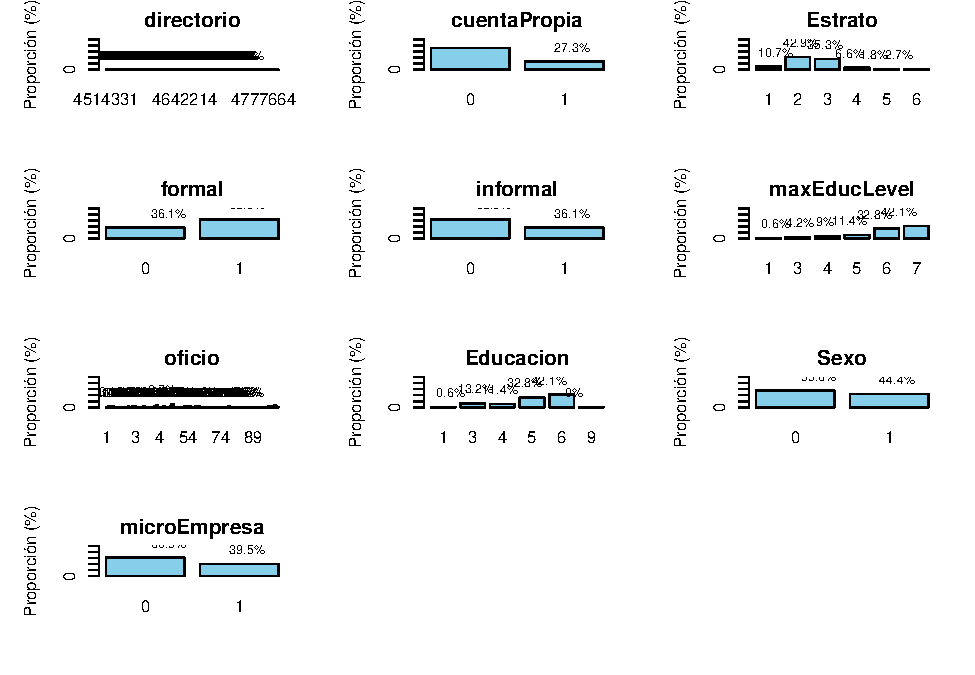
\includegraphics{Taller-1_files/figure-latex/unnamed-chunk-13-1.pdf}

La distribución individual de las variables cuantitativas se muestra a
continuación. El comportamiento de la edad es bastante uniforme y la
mayor concentración se encuentra alrededor de los 37 años. Siguiendo la
teoría del ciclo de vida, la mayoría de las personas encuestadas se
encuentran en una edad adulta temprana. En el aspecto laboral, esto
significa que ya se encuentran en un momento de estabilidad y donde son
más productivas, y los salarios deberían ser más altos ya que se cuenta
con más experiencia.

Este argumento se contrasta con los datos de experiencia en su trabajo,
que se miden a partir de los meses que llevan trabajando en la misma
empresa. Los datos muestran que, en promedio, las personas llevan
trabajando en el mismo lugar 5 años. Sin embargo, la diferencia con la
mediana es muy alta, ya que el valor medio de los meses trabajados es 2
años. Esta distorsión se puede explicar por la presencia de datos
atípicos.

Por el lado de las horas trabajadas la semana pasada, sus valores están
muy cercanos a las exigidas por la legislación laboral colombiana.

\begin{Shaded}
\begin{Highlighting}[]
\NormalTok{quantitative\_vars }\OtherTok{\textless{}{-}}\NormalTok{ data\_h }\SpecialCharTok{\%\textgreater{}\%}
  \FunctionTok{select}\NormalTok{(}\FunctionTok{where}\NormalTok{(is.numeric))}

\NormalTok{plot\_histogram }\OtherTok{\textless{}{-}} \ControlFlowTok{function}\NormalTok{(column, col\_name) \{}
  \FunctionTok{hist}\NormalTok{(column, }\AttributeTok{main =}\NormalTok{ col\_name, }\AttributeTok{xlab =}\NormalTok{ col\_name, }\AttributeTok{ylab =} \StringTok{"Frecuencia"}\NormalTok{, }\AttributeTok{col =} \StringTok{"skyblue"}\NormalTok{)}
\NormalTok{\}}

\NormalTok{num\_vars }\OtherTok{\textless{}{-}} \FunctionTok{ncol}\NormalTok{(quantitative\_vars)}
\NormalTok{num\_rows }\OtherTok{\textless{}{-}} \FunctionTok{ceiling}\NormalTok{(}\FunctionTok{sqrt}\NormalTok{(num\_vars))}
\NormalTok{num\_cols }\OtherTok{\textless{}{-}} \FunctionTok{ceiling}\NormalTok{(num\_vars }\SpecialCharTok{/}\NormalTok{ num\_rows)}

\FunctionTok{par}\NormalTok{(}\AttributeTok{mfrow =} \FunctionTok{c}\NormalTok{(num\_rows, num\_cols), }\AttributeTok{mar =} \FunctionTok{c}\NormalTok{(}\DecValTok{5}\NormalTok{, }\DecValTok{5}\NormalTok{, }\DecValTok{2}\NormalTok{, }\DecValTok{2}\NormalTok{))  }

\FunctionTok{walk2}\NormalTok{(quantitative\_vars, }\FunctionTok{names}\NormalTok{(quantitative\_vars), plot\_histogram)}
\end{Highlighting}
\end{Shaded}

\includegraphics{Taller-1_files/figure-latex/unnamed-chunk-14-1.pdf}

\hypertarget{anuxe1lisis-exploratorio-bivariado}{%
\subsection{Análisis exploratorio
bivariado}\label{anuxe1lisis-exploratorio-bivariado}}

\hfill\break
En este apartado se explorarán las diferencias que pueden existir entre
las categorías analizadas en la sección anterior cuando se presentan a
través del logaritmo del salario. Las diferencias más grandes se
observan a través de la variable Estrato Socioeconómico y en el nivel de
educación cuando el encuestado cuenta con grado de educación superior.

Las diferencias a través del estrato se intuyen por la naturaleza de
esta variable, ya que mide, entre otras cosas, la capacidad adquisitiva
del hogar. Mientras tanto, el tema del estudio se explica por la teoría
del capital humano, que sostiene que la formación de los individuos son
inversiones que aumentan su productividad e ingresos a lo largo del
tiempo.

Se observan diferencias moderadas a través de variables como si el
encuestado trabaja por cuenta propia o si está desempeñando su trabajo
en condiciones de informalidad. Los datos muestran un ligero aumento del
salario promedio si la persona trabaja como empleada. Además, los
trabajadores que trabajan como empleados formales perciben unos ingresos
ligeramente mayores que los trabajadores informales. No se observan
diferencias en el caso del sexo, donde los salarios son uniformes para
hombres y mujeres.

\begin{Shaded}
\begin{Highlighting}[]
\FunctionTok{options}\NormalTok{(}\AttributeTok{repr.plot.width =} \DecValTok{20}\NormalTok{, }\AttributeTok{repr.plot.height =} \DecValTok{10}\NormalTok{)}
\NormalTok{qualitative\_vars }\OtherTok{\textless{}{-}}\NormalTok{ data\_h }\SpecialCharTok{\%\textgreater{}\%} \FunctionTok{select}\NormalTok{(}\FunctionTok{where}\NormalTok{(is.factor) }\SpecialCharTok{|} \FunctionTok{where}\NormalTok{(is.character))}
\end{Highlighting}
\end{Shaded}

\begin{verbatim}
## Adding missing grouping variables: `directorio`
\end{verbatim}

\begin{Shaded}
\begin{Highlighting}[]
\NormalTok{num\_cols }\OtherTok{\textless{}{-}} \DecValTok{4}
\NormalTok{num\_rows }\OtherTok{\textless{}{-}} \FunctionTok{ceiling}\NormalTok{(}\FunctionTok{ncol}\NormalTok{(qualitative\_vars) }\SpecialCharTok{/}\NormalTok{ num\_cols)}
\FunctionTok{par}\NormalTok{(}\AttributeTok{mfrow =} \FunctionTok{c}\NormalTok{(num\_rows, num\_cols))}
\ControlFlowTok{for}\NormalTok{ (col }\ControlFlowTok{in} \FunctionTok{colnames}\NormalTok{(qualitative\_vars)) \{}
  \FunctionTok{suppressWarnings}\NormalTok{(}\FunctionTok{boxplot}\NormalTok{(log\_salario }\SpecialCharTok{\textasciitilde{}}\NormalTok{ data\_h[[col]], }\AttributeTok{data =}\NormalTok{ data\_h, }\AttributeTok{main =}\NormalTok{ col, }\AttributeTok{xlab =}\NormalTok{ col, }\AttributeTok{ylab =} \StringTok{"log\_salario"}\NormalTok{))}
\NormalTok{\}}
\end{Highlighting}
\end{Shaded}

\includegraphics{Taller-1_files/figure-latex/unnamed-chunk-15-1.pdf}

En relación a las variables de naturaleza cuantitativa, no se observan
patrones que ayuden a determinar cambios significativos en el ingreso
laboral. Incluso, los niveles de correlación entre las variables no
muestran señales de que puedan aportar cuando se inicie con el proceso
de modelación.

\begin{Shaded}
\begin{Highlighting}[]
\FunctionTok{options}\NormalTok{(}\AttributeTok{repr.plot.width =} \DecValTok{20}\NormalTok{, }\AttributeTok{repr.plot.height =} \DecValTok{10}\NormalTok{)}

\CommentTok{\# Seleccionar variables cuantitativas}
\NormalTok{numeric\_vars }\OtherTok{\textless{}{-}}\NormalTok{ data\_h }\SpecialCharTok{\%\textgreater{}\%} \FunctionTok{select}\NormalTok{(}\FunctionTok{where}\NormalTok{(is.numeric))}

\CommentTok{\# Establecer el número de columnas para la disposición de la grilla}
\NormalTok{num\_cols }\OtherTok{\textless{}{-}} \DecValTok{4}
\NormalTok{num\_rows }\OtherTok{\textless{}{-}} \FunctionTok{ceiling}\NormalTok{(}\FunctionTok{ncol}\NormalTok{(numeric\_vars) }\SpecialCharTok{/}\NormalTok{ num\_cols)}

\CommentTok{\# Establecer el tamaño de la gráfica}
\FunctionTok{par}\NormalTok{(}\AttributeTok{mfrow =} \FunctionTok{c}\NormalTok{(num\_rows, num\_cols))}

\CommentTok{\# Crear scatter plots para variables cuantitativas}
\ControlFlowTok{for}\NormalTok{ (col }\ControlFlowTok{in} \FunctionTok{colnames}\NormalTok{(numeric\_vars)) \{}
  \FunctionTok{suppressWarnings}\NormalTok{(}\FunctionTok{plot}\NormalTok{(data\_h[[col]], data\_h}\SpecialCharTok{$}\NormalTok{log\_salario, }\AttributeTok{main =}\NormalTok{ col, }\AttributeTok{xlab =}\NormalTok{ col, }\AttributeTok{ylab =} \StringTok{"log\_salario"}\NormalTok{))}
\NormalTok{\}}
\end{Highlighting}
\end{Shaded}

\includegraphics{Taller-1_files/figure-latex/unnamed-chunk-16-1.pdf}

\hypertarget{anuxe1lisis-de-regresion}{%
\section{3. Análisis de regresion}\label{anuxe1lisis-de-regresion}}

EL propósito es estimar el siguiente modelo:

\[log(w) = \beta_{1} + \beta_{2}Edad + \beta_{3}Edad^2\]

\begin{Shaded}
\begin{Highlighting}[]
\NormalTok{modelo1}\OtherTok{\textless{}{-}}\FunctionTok{lm}\NormalTok{(log\_salario }\SpecialCharTok{\textasciitilde{}}\NormalTok{  Edad }\SpecialCharTok{+}\NormalTok{ Edad2,}
\AttributeTok{data=}\NormalTok{data\_h)}
\NormalTok{stargazer}\SpecialCharTok{::}\FunctionTok{stargazer}\NormalTok{(modelo1,}\AttributeTok{type =} \StringTok{"text"}\NormalTok{)}
\end{Highlighting}
\end{Shaded}

\begin{verbatim}
## 
## ===============================================
##                         Dependent variable:    
##                     ---------------------------
##                             log_salario        
## -----------------------------------------------
## Edad                         0.064***          
##                               (0.003)          
##                                                
## Edad2                        -0.001***         
##                              (0.00004)         
##                                                
## Constant                     12.786***         
##                               (0.060)          
##                                                
## -----------------------------------------------
## Observations                  13,786           
## R2                             0.032           
## Adjusted R2                    0.032           
## Residual Std. Error     0.754 (df = 13783)     
## F Statistic         229.589*** (df = 2; 13783) 
## ===============================================
## Note:               *p<0.1; **p<0.05; ***p<0.01
\end{verbatim}

Los coeficientes de la regresión son significativos hasta a un nivel de
confianza del 95\%. A partir de ellos podemos rescatar la siguiente
ecuación de salarios en función de la edad

\[log(w) = 12.786 + 0.64 Edad - 0.001 Edad^2 + u\]

Se evidencia que el ajuste del modelo dentro de la muestra no es muy
grande ya que el R2 es de 0.032. Esta medida también la podemos
complementar con el cálculo el error cuadrático medio MSE.

\begin{Shaded}
\begin{Highlighting}[]
\NormalTok{fit}\OtherTok{\textless{}{-}}\FunctionTok{predict.lm}\NormalTok{(modelo1,}\AttributeTok{newdata =}\NormalTok{ data\_h)}
\NormalTok{data\_h}\SpecialCharTok{$}\NormalTok{log\_salario\_gorro}\OtherTok{\textless{}{-}}\NormalTok{fit}
\NormalTok{MSE}\OtherTok{\textless{}{-}}\FunctionTok{sum}\NormalTok{((data\_h}\SpecialCharTok{$}\NormalTok{log\_salario}\SpecialCharTok{{-}}\NormalTok{data\_h}\SpecialCharTok{$}\NormalTok{log\_salario\_gorro)}\SpecialCharTok{\^{}}\DecValTok{2}\NormalTok{)}\SpecialCharTok{/}\FunctionTok{length}\NormalTok{(data\_h}\SpecialCharTok{$}\NormalTok{log\_salario)}
\NormalTok{MSE}
\end{Highlighting}
\end{Shaded}

\begin{verbatim}
## [1] 0.568164
\end{verbatim}

Aumentando la complejidad del modelo es probable que tanto el R2 aumente
como el MSE se reduzca, sin embargo, con esto estaremos aumentando la
varianza de los estimadores, lo que permite disminuir el sesgo.

A partir de los coeficientes obtenidos es posible calcular la edad pico
en el crecimiento de los ingresos de las personas.

\[\frac {\partial log(w)}{\partial Edad} =0 \]

\[\frac {\partial log(w)}{\partial Edad} = \beta 1-(2) \beta2Edad=0\]

\[Edad^*=\frac {\beta1}{-(2)\beta 2}\]

Calculamos la edad pico, al tiempo que construimos la función que nos
permitirá mediante el bootstrap estimar la varianza de los estimadores
para la generación del intérvalo de confianza.

\begin{Shaded}
\begin{Highlighting}[]
\NormalTok{bfuncion}\OtherTok{\textless{}{-}}\ControlFlowTok{function}\NormalTok{(data,index)\{}
  
\NormalTok{modelo}\OtherTok{\textless{}{-}}\FunctionTok{lm}\NormalTok{(log\_salario }\SpecialCharTok{\textasciitilde{}}\NormalTok{  Edad }\SpecialCharTok{+}\NormalTok{ Edad2, }\AttributeTok{data=}\NormalTok{data\_h,}\AttributeTok{subset =}\NormalTok{ index)}

\NormalTok{coeficientes}\OtherTok{\textless{}{-}}\NormalTok{modelo}\SpecialCharTok{$}\NormalTok{coefficients}

\NormalTok{b1}\OtherTok{\textless{}{-}}\NormalTok{coeficientes[}\DecValTok{2}\NormalTok{]}
\NormalTok{b2}\OtherTok{\textless{}{-}}\NormalTok{coeficientes[}\DecValTok{3}\NormalTok{]}

\NormalTok{edad\_pico}\OtherTok{\textless{}{-}}\NormalTok{b1}\SpecialCharTok{/}\NormalTok{(}\SpecialCharTok{{-}}\DecValTok{2}\SpecialCharTok{*}\NormalTok{b2)}
\FunctionTok{return}\NormalTok{(edad\_pico) }\CommentTok{\#returns the second coefficient of the linear regression}
\NormalTok{\}}

\NormalTok{edad\_pico}\OtherTok{\textless{}{-}}\FunctionTok{bfuncion}\NormalTok{(data\_h,}\DecValTok{1}\SpecialCharTok{:}\FunctionTok{nrow}\NormalTok{(data\_h))}
\NormalTok{modelo1}\SpecialCharTok{$}\NormalTok{coefficients[}\DecValTok{2}\NormalTok{]}\SpecialCharTok{/}\NormalTok{(}\SpecialCharTok{{-}}\DecValTok{2}\SpecialCharTok{*}\NormalTok{modelo1}\SpecialCharTok{$}\NormalTok{coefficients[}\DecValTok{3}\NormalTok{])}
\end{Highlighting}
\end{Shaded}

\begin{verbatim}
##     Edad 
## 41.93591
\end{verbatim}

\begin{Shaded}
\begin{Highlighting}[]
\NormalTok{edad\_pico}
\end{Highlighting}
\end{Shaded}

\begin{verbatim}
##     Edad 
## 41.93591
\end{verbatim}

Para poder realizar esta inferencia calculamos la Varianza utilizando
bootstap.

\begin{Shaded}
\begin{Highlighting}[]
\FunctionTok{set.seed}\NormalTok{(}\DecValTok{123}\NormalTok{)}
\NormalTok{repeticiones}\OtherTok{\textless{}{-}}\DecValTok{1000}
\FunctionTok{boot}\NormalTok{(data\_h,bfuncion,}\AttributeTok{R=}\NormalTok{repeticiones)}
\end{Highlighting}
\end{Shaded}

\begin{verbatim}
## 
## ORDINARY NONPARAMETRIC BOOTSTRAP
## 
## 
## Call:
## boot(data = data_h, statistic = bfuncion, R = repeticiones)
## 
## 
## Bootstrap Statistics :
##     original        bias    std. error
## t1* 41.93591 -2.638615e-05   0.3462259
\end{verbatim}

Con esto podemos establecer el intervalo de confianza para la edad pico

\[Edad^* \pm t_{\alpha/2} * 0.3462259\]

Es decir que para un nivel de confianza del 95\%

\begin{Shaded}
\begin{Highlighting}[]
\NormalTok{n}\OtherTok{=}\FunctionTok{nrow}\NormalTok{(}\AttributeTok{x =}\NormalTok{ data\_h)}
\NormalTok{t}\OtherTok{=}\FunctionTok{abs}\NormalTok{(}\FunctionTok{qt}\NormalTok{(}\AttributeTok{p =}\NormalTok{ (}\DecValTok{1}\FloatTok{{-}0.95}\NormalTok{)}\SpecialCharTok{/}\DecValTok{2}\NormalTok{,}\AttributeTok{df =}\NormalTok{n}\DecValTok{{-}1}\NormalTok{ ))}
\NormalTok{limite\_inferior}\OtherTok{=}\NormalTok{edad\_pico}\SpecialCharTok{{-}}\NormalTok{(t}\SpecialCharTok{*}\FloatTok{0.3462259}\NormalTok{)}
\NormalTok{limite\_superior}\OtherTok{=}\NormalTok{edad\_pico}\SpecialCharTok{+}\NormalTok{(t}\SpecialCharTok{*}\FloatTok{0.3462259}\NormalTok{)}
\NormalTok{limites}\OtherTok{\textless{}{-}}\FunctionTok{c}\NormalTok{(limite\_inferior,limite\_superior)}
\NormalTok{limites}
\end{Highlighting}
\end{Shaded}

\begin{verbatim}
##     Edad     Edad 
## 41.25726 42.61456
\end{verbatim}

Observamos de manera gráfica el ajuste del modelo a los datos.

\begin{Shaded}
\begin{Highlighting}[]
\NormalTok{data\_aux}\OtherTok{\textless{}{-}}\NormalTok{data\_h }\SpecialCharTok{\%\textgreater{}\%} \FunctionTok{select}\NormalTok{(log\_salario,log\_salario\_gorro,Edad)}
\end{Highlighting}
\end{Shaded}

\begin{verbatim}
## Adding missing grouping variables: `directorio`
\end{verbatim}

\begin{Shaded}
\begin{Highlighting}[]
\NormalTok{data\_aux}\OtherTok{\textless{}{-}}\NormalTok{data\_aux }\SpecialCharTok{\%\textgreater{}\%}  \FunctionTok{pivot\_longer}\NormalTok{(}\AttributeTok{cols =}\NormalTok{ log\_salario}\SpecialCharTok{:}\NormalTok{log\_salario\_gorro,}
\AttributeTok{names\_to =} \StringTok{"Predict"}\NormalTok{,}
\AttributeTok{values\_to =} \StringTok{"Valor"}\NormalTok{)}

\FunctionTok{ggplot}\NormalTok{(data\_aux,}\FunctionTok{aes}\NormalTok{(}\AttributeTok{x=}\NormalTok{Edad,}\AttributeTok{color=}\NormalTok{Predict)) }\SpecialCharTok{+}
\FunctionTok{geom\_point}\NormalTok{(}\FunctionTok{aes}\NormalTok{(}\AttributeTok{y=}\NormalTok{Valor)) }\SpecialCharTok{+}
\FunctionTok{labs}\NormalTok{(}\AttributeTok{title =} \StringTok{"Ajuste del modelo a los datos de la muestra"}\NormalTok{,}
\AttributeTok{x=}\StringTok{"Edad"}\NormalTok{,}
\AttributeTok{y=}\StringTok{"Log salario"}
\NormalTok{) }\SpecialCharTok{+}
\FunctionTok{theme\_stata}\NormalTok{() }\SpecialCharTok{+}
\FunctionTok{scale\_fill\_stata}\NormalTok{()}
\end{Highlighting}
\end{Shaded}

\includegraphics{Taller-1_files/figure-latex/unnamed-chunk-22-1.pdf}

\hypertarget{modelo-de-guxe9nero}{%
\section{4. Modelo de género}\label{modelo-de-guxe9nero}}

\[log(w) = \beta_{1} + \beta_{2}Mujer\]a) Estimación del modelo general.

\begin{Shaded}
\begin{Highlighting}[]
\NormalTok{modelS}\OtherTok{\textless{}{-}}\FunctionTok{lm}\NormalTok{(log\_salario }\SpecialCharTok{\textasciitilde{}}\NormalTok{Sexo,}\AttributeTok{data=}\NormalTok{data\_h)}
\NormalTok{stargazer}\SpecialCharTok{::}\FunctionTok{stargazer}\NormalTok{(modelS,}\AttributeTok{type =} \StringTok{"text"}\NormalTok{)}
\end{Highlighting}
\end{Shaded}

\begin{verbatim}
## 
## ===============================================
##                         Dependent variable:    
##                     ---------------------------
##                             log_salario        
## -----------------------------------------------
## Sexo1                        -0.096***         
##                               (0.013)          
##                                                
## Constant                     14.046***         
##                               (0.009)          
##                                                
## -----------------------------------------------
## Observations                  13,786           
## R2                             0.004           
## Adjusted R2                    0.004           
## Residual Std. Error     0.765 (df = 13784)     
## F Statistic          53.854*** (df = 1; 13784) 
## ===============================================
## Note:               *p<0.1; **p<0.05; ***p<0.01
\end{verbatim}

En el modelo general, al estimar el logaritmo natural del salario contra
el sexo de la persona, se observa que las mujeres, en promedio, ganan
menos que los hombres. La relación es estadísticamente significativa y
el parámetro -0.068 indica que por ser mujer se espera que el logaritmo
natural del salario disminuya 0.068 unidades en promedio. Esta relación
es estadísticamente significativa y valida la hipótesis muy trabajada en
el mercado laboral que muestra que hay diferencias significativas en las
ganancias entre hombres y mujeres.

Aplicación del teorema FWL:

Para la aplicación del teorema de FWL se siguen dos pasos. En primer
lugar, se estima un modelo donde la variable de interés, en este caso el
género de la persona encuestada, se deja como variable independiente
frente a las variables de control y se toman los residuales.

Luego se estima el segundo modelo donde la variable independiente es el
logaritmo del salario frente a las variables de control y se toman los
residuales. Por último, se estima la regresión de los dos residuales.

Se espera que el parámetro estimado en el primer modelo sea igual a la
estimación del modelo en los residuales.

Para esto se incluyen las siguientes variables de control:

\begin{itemize}
\item
  Edad
\item
  Oficio
\item
  Si trabaja en microempresa
\item
  Educación formal
\end{itemize}

El objetivo de esta estimación no es encontrar los determinantes del
salario como se hizo en la primera parte, sino entender las diferencias
en salario que se pueden presentar a través del sexo de las personas.
Por esto se incluyeron estas variables que pueden controlar mejor el
sesgo de solo incluir el sexo.

Paso 1: Estimar la ecuación del género de las personas contra las
variables de control y tomar los residuales.

\begin{Shaded}
\begin{Highlighting}[]
\NormalTok{resid1 }\OtherTok{\textless{}{-}} \FunctionTok{lm}\NormalTok{(Sexo }\SpecialCharTok{\textasciitilde{}}\NormalTok{Estrato}\SpecialCharTok{+}\NormalTok{oficio}\SpecialCharTok{+}\NormalTok{Edad}\SpecialCharTok{+}\NormalTok{Edad2}\SpecialCharTok{+}\NormalTok{informal}\SpecialCharTok{+}\NormalTok{maxEducLevel}\SpecialCharTok{+}\NormalTok{microEmpresa,}\AttributeTok{data =}\NormalTok{ data\_h)}\SpecialCharTok{$}\NormalTok{residuals}
\end{Highlighting}
\end{Shaded}

Paso 2: Se estima el salario solo frente a las variables de control y se
toman los residuales.

\begin{Shaded}
\begin{Highlighting}[]
\NormalTok{resid2 }\OtherTok{=} \FunctionTok{lm}\NormalTok{(log\_salario }\SpecialCharTok{\textasciitilde{}}\NormalTok{Estrato}\SpecialCharTok{+}\NormalTok{oficio}\SpecialCharTok{+}\NormalTok{Edad}\SpecialCharTok{+}\NormalTok{Edad2}\SpecialCharTok{+}\NormalTok{informal}\SpecialCharTok{+}\NormalTok{maxEducLevel}\SpecialCharTok{+}\NormalTok{microEmpresa,}\AttributeTok{data =}\NormalTok{ data\_h)}\SpecialCharTok{$}\NormalTok{residuals}
\end{Highlighting}
\end{Shaded}

\begin{Shaded}
\begin{Highlighting}[]
\NormalTok{general}\OtherTok{\textless{}{-}}\FunctionTok{lm}\NormalTok{(log\_salario }\SpecialCharTok{\textasciitilde{}}\NormalTok{Estrato}\SpecialCharTok{+}\NormalTok{oficio}\SpecialCharTok{+}\NormalTok{Edad}\SpecialCharTok{+}\NormalTok{Edad2}\SpecialCharTok{+}\NormalTok{informal}\SpecialCharTok{+}\NormalTok{maxEducLevel}\SpecialCharTok{+}\NormalTok{microEmpresa}\SpecialCharTok{+}\NormalTok{Sexo,}\AttributeTok{data =}\NormalTok{ data\_h)}
\NormalTok{mod\_resid}\OtherTok{=}\FunctionTok{lm}\NormalTok{(resid2}\SpecialCharTok{\textasciitilde{}}\NormalTok{resid1)}
\end{Highlighting}
\end{Shaded}

\begin{Shaded}
\begin{Highlighting}[]
\NormalTok{stargazer}\SpecialCharTok{::}\FunctionTok{stargazer}\NormalTok{(general,mod\_resid,modelS,}\AttributeTok{type =} \StringTok{"text"}\NormalTok{,}\AttributeTok{digits=} \DecValTok{3}\NormalTok{)}
\end{Highlighting}
\end{Shaded}

\begin{verbatim}
## 
## ====================================================================================================
##                                                   Dependent variable:                               
##                     --------------------------------------------------------------------------------
##                             log_salario                   resid2                  log_salario       
##                                 (1)                        (2)                        (3)           
## ----------------------------------------------------------------------------------------------------
## Estrato2                      0.026*                                                                
##                               (0.016)                                                               
##                                                                                                     
## Estrato3                     0.137***                                                               
##                               (0.017)                                                               
##                                                                                                     
## Estrato4                     0.536***                                                               
##                               (0.025)                                                               
##                                                                                                     
## Estrato5                     0.763***                                                               
##                               (0.038)                                                               
##                                                                                                     
## Estrato6                     1.119***                                                               
##                               (0.034)                                                               
##                                                                                                     
## oficio11                     -0.267**                                                               
##                               (0.127)                                                               
##                                                                                                     
## oficio12                      -0.079                                                                
##                               (0.127)                                                               
##                                                                                                     
## oficio13                     -0.388***                                                              
##                               (0.124)                                                               
##                                                                                                     
## oficio14                     -0.958***                                                              
##                               (0.267)                                                               
##                                                                                                     
## oficio15                     -0.329**                                                               
##                               (0.143)                                                               
##                                                                                                     
## oficio16                     -0.644***                                                              
##                               (0.131)                                                               
##                                                                                                     
## oficio17                     -0.599***                                                              
##                               (0.149)                                                               
##                                                                                                     
## oficio18                     -0.820***                                                              
##                               (0.149)                                                               
##                                                                                                     
## oficio19                     -0.458***                                                              
##                               (0.128)                                                               
##                                                                                                     
## oficio2                       -0.223*                                                               
##                               (0.126)                                                               
##                                                                                                     
## oficio20                       0.036                                                                
##                               (0.544)                                                               
##                                                                                                     
## oficio21                      -0.176                                                                
##                               (0.124)                                                               
##                                                                                                     
## oficio3                      -0.708***                                                              
##                               (0.124)                                                               
##                                                                                                     
## oficio30                     -0.310**                                                               
##                               (0.132)                                                               
##                                                                                                     
## oficio31                       0.063                                                                
##                               (0.187)                                                               
##                                                                                                     
## oficio32                     -0.679***                                                              
##                               (0.132)                                                               
##                                                                                                     
## oficio33                     -0.693***                                                              
##                               (0.125)                                                               
##                                                                                                     
## oficio34                     -0.867***                                                              
##                               (0.142)                                                               
##                                                                                                     
## oficio35                     -0.760***                                                              
##                               (0.207)                                                               
##                                                                                                     
## oficio36                     -1.192***                                                              
##                               (0.151)                                                               
##                                                                                                     
## oficio37                     -0.910***                                                              
##                               (0.130)                                                               
##                                                                                                     
## oficio38                     -0.850***                                                              
##                               (0.127)                                                               
##                                                                                                     
## oficio39                     -0.711***                                                              
##                               (0.123)                                                               
##                                                                                                     
## oficio4                       0.517*                                                                
##                               (0.292)                                                               
##                                                                                                     
## oficio40                     -0.557***                                                              
##                               (0.146)                                                               
##                                                                                                     
## oficio41                     -0.648***                                                              
##                               (0.124)                                                               
##                                                                                                     
## oficio42                     -0.549***                                                              
##                               (0.142)                                                               
##                                                                                                     
## oficio43                      -0.201                                                                
##                               (0.180)                                                               
##                                                                                                     
## oficio44                     -0.544***                                                              
##                               (0.127)                                                               
##                                                                                                     
## oficio45                     -0.790***                                                              
##                               (0.123)                                                               
##                                                                                                     
## oficio49                     -0.619**                                                               
##                               (0.267)                                                               
##                                                                                                     
## oficio5                       -0.161                                                                
##                               (0.157)                                                               
##                                                                                                     
## oficio50                     -0.555***                                                              
##                               (0.156)                                                               
##                                                                                                     
## oficio51                     -0.555***                                                              
##                               (0.135)                                                               
##                                                                                                     
## oficio52                     -0.776***                                                              
##                               (0.235)                                                               
##                                                                                                     
## oficio53                     -0.804***                                                              
##                               (0.124)                                                               
##                                                                                                     
## oficio54                     -1.002***                                                              
##                               (0.125)                                                               
##                                                                                                     
## oficio55                     -0.899***                                                              
##                               (0.125)                                                               
##                                                                                                     
## oficio56                     -0.853***                                                              
##                               (0.151)                                                               
##                                                                                                     
## oficio57                     -0.792***                                                              
##                               (0.129)                                                               
##                                                                                                     
## oficio58                     -0.673***                                                              
##                               (0.124)                                                               
##                                                                                                     
## oficio59                     -0.775***                                                              
##                               (0.125)                                                               
##                                                                                                     
## oficio6                       -0.234*                                                               
##                               (0.131)                                                               
##                                                                                                     
## oficio60                     -2.516***                                                              
##                               (0.544)                                                               
##                                                                                                     
## oficio61                     -0.623***                                                              
##                               (0.180)                                                               
##                                                                                                     
## oficio62                     -0.809***                                                              
##                               (0.153)                                                               
##                                                                                                     
## oficio63                      -0.489                                                                
##                               (0.395)                                                               
##                                                                                                     
## oficio7                      -0.416***                                                              
##                               (0.136)                                                               
##                                                                                                     
## oficio70                     -0.459***                                                              
##                               (0.141)                                                               
##                                                                                                     
## oficio72                     -0.717***                                                              
##                               (0.224)                                                               
##                                                                                                     
## oficio73                      -0.056                                                                
##                               (0.395)                                                               
##                                                                                                     
## oficio74                     -0.708***                                                              
##                               (0.201)                                                               
##                                                                                                     
## oficio75                     -1.244***                                                              
##                               (0.168)                                                               
##                                                                                                     
## oficio76                     -0.698**                                                               
##                               (0.330)                                                               
##                                                                                                     
## oficio77                     -0.680***                                                              
##                               (0.129)                                                               
##                                                                                                     
## oficio79                     -0.836***                                                              
##                               (0.125)                                                               
##                                                                                                     
## oficio8                       -0.144                                                                
##                               (0.129)                                                               
##                                                                                                     
## oficio80                     -0.967***                                                              
##                               (0.134)                                                               
##                                                                                                     
## oficio81                     -0.886***                                                              
##                               (0.135)                                                               
##                                                                                                     
## oficio82                     -1.136***                                                              
##                               (0.395)                                                               
##                                                                                                     
## oficio83                     -0.761***                                                              
##                               (0.133)                                                               
##                                                                                                     
## oficio84                     -0.720***                                                              
##                               (0.128)                                                               
##                                                                                                     
## oficio85                     -0.670***                                                              
##                               (0.129)                                                               
##                                                                                                     
## oficio86                      -0.528                                                                
##                               (0.330)                                                               
##                                                                                                     
## oficio87                     -0.741***                                                              
##                               (0.130)                                                               
##                                                                                                     
## oficio88                     -0.851***                                                              
##                               (0.249)                                                               
##                                                                                                     
## oficio89                     -0.741***                                                              
##                               (0.170)                                                               
##                                                                                                     
## oficio9                       -0.093                                                                
##                               (0.140)                                                               
##                                                                                                     
## oficio90                     -0.808***                                                              
##                               (0.141)                                                               
##                                                                                                     
## oficio91                     -0.809***                                                              
##                               (0.208)                                                               
##                                                                                                     
## oficio92                     -0.667***                                                              
##                               (0.145)                                                               
##                                                                                                     
## oficio93                     -0.776***                                                              
##                               (0.133)                                                               
##                                                                                                     
## oficio94                     -0.993***                                                              
##                               (0.163)                                                               
##                                                                                                     
## oficio95                     -0.671***                                                              
##                               (0.124)                                                               
##                                                                                                     
## oficio96                      -0.077                                                                
##                               (0.395)                                                               
##                                                                                                     
## oficio97                     -0.870***                                                              
##                               (0.125)                                                               
##                                                                                                     
## oficio98                     -0.682***                                                              
##                               (0.124)                                                               
##                                                                                                     
## oficio99                     -0.859***                                                              
##                               (0.134)                                                               
##                                                                                                     
## Edad                         0.046***                                                               
##                               (0.002)                                                               
##                                                                                                     
## Edad2                        -0.001***                                                              
##                              (0.00003)                                                              
##                                                                                                     
## informal1                    -0.241***                                                              
##                               (0.013)                                                               
##                                                                                                     
## maxEducLevel3                  0.094                                                                
##                               (0.063)                                                               
##                                                                                                     
## maxEducLevel4                 0.152**                                                               
##                               (0.061)                                                               
##                                                                                                     
## maxEducLevel5                0.201***                                                               
##                               (0.061)                                                               
##                                                                                                     
## maxEducLevel6                0.254***                                                               
##                               (0.061)                                                               
##                                                                                                     
## maxEducLevel7                0.414***                                                               
##                               (0.061)                                                               
##                                                                                                     
## microEmpresa1                -0.208***                                                              
##                               (0.013)                                                               
##                                                                                                     
## Sexo1                        -0.129***                                             -0.096***        
##                               (0.011)                                               (0.013)         
##                                                                                                     
## resid1                                                  -0.129***                                   
##                                                          (0.011)                                    
##                                                                                                     
## Constant                     13.531***                    -0.000                   14.046***        
##                               (0.144)                    (0.005)                    (0.009)         
##                                                                                                     
## ----------------------------------------------------------------------------------------------------
## Observations                  13,786                      13,786                    13,786          
## R2                             0.524                      0.010                      0.004          
## Adjusted R2                    0.521                      0.010                      0.004          
## Residual Std. Error     0.530 (df = 13692)          0.528 (df = 13784)        0.765 (df = 13784)    
## F Statistic         162.314*** (df = 93; 13692) 139.317*** (df = 1; 13784) 53.854*** (df = 1; 13784)
## ====================================================================================================
## Note:                                                                    *p<0.1; **p<0.05; ***p<0.01
\end{verbatim}

Luego de aplicar el teorema de FWL se observa cómo los coeficientes
estimados son iguales, por lo que se valida utilizar las variables de
control que se han venido trabajando.

A través de las tres especificaciones se ha comprobado que existen
diferencias en el salario entre hombres y mujeres. Desde la estimación
se observa que las mujeres, en promedio, ganan menos que los hombres en
condiciones de empleo iguales. En el primer modelo general, cuando no se
incluyen variables de control, se nota cómo en promedio las mujeres
ganan 0.06 unidades menos que los hombres, y cuando se incluyen
variables de control la diferencia es de 0.09 unidades en el logaritmo
del salario.

\hypertarget{predicciuxf3n}{%
\section{5 Predicción}\label{predicciuxf3n}}

Las especificaciones que se van a trabajar para el proceso de predicción
se van a construir tomando como referencia la ecuación de Mincer.

\[Ln(w) = \beta_{0} +* \beta_{1}S + \beta_{2}Exp +* \beta_{3}Exp^2 +
\epsilon\]

\begin{enumerate}
\def\labelenumi{\arabic{enumi}.}
\setcounter{enumi}{1}
\tightlist
\item
  Tomando los elementos de la ecuacion de mince pero anadiendo las
  variables propuestas desde el punto de vista empirico
\end{enumerate}

\[Ln(w) = \beta_{0} + \beta_{1}Edad + \beta_{2}edad^2 + \beta_{3}Cuentapropia + +\beta_{4}Estrato+ \beta_{5}informal+ \beta_{6}Educacion + \beta_{7}sexo+ \beta_{8}Microempresa+ \beta_{9}Horas_trabajadas + \beta_{10}oficio +\epsilon\]

\begin{enumerate}
\def\labelenumi{\arabic{enumi}.}
\setcounter{enumi}{2}
\tightlist
\item
  Modelo del punto 3 donde solo se tenia en cuenta la edad
\end{enumerate}

\[ ln(w)=\beta_{0} + \beta_{1}Edad + \beta_{2}edad^2 \]

Luego de estas estimaciones se estiman otros modelos derivados de los
generales, aplicando alguna complejidad al modelo y poder estimar de
mejor forma los determinantes del salario.

\begin{enumerate}
\def\labelenumi{\alph{enumi})}
\tightlist
\item
  Particion de los datos
\end{enumerate}

\begin{Shaded}
\begin{Highlighting}[]
\FunctionTok{set.seed}\NormalTok{(}\DecValTok{10101}\NormalTok{)}

\NormalTok{train\_size }\OtherTok{\textless{}{-}} \FunctionTok{floor}\NormalTok{(}\FloatTok{0.7} \SpecialCharTok{*} \FunctionTok{nrow}\NormalTok{(data\_h))}


\NormalTok{train\_indices }\OtherTok{\textless{}{-}} \FunctionTok{sample}\NormalTok{(}\DecValTok{1}\SpecialCharTok{:}\FunctionTok{nrow}\NormalTok{(data\_h), }\AttributeTok{size =}\NormalTok{ train\_size, }\AttributeTok{replace =} \ConstantTok{FALSE}\NormalTok{)}


\NormalTok{train }\OtherTok{\textless{}{-}}\NormalTok{ data\_h[train\_indices, ]}


\NormalTok{test }\OtherTok{\textless{}{-}}\NormalTok{ data\_h }\SpecialCharTok{\%\textgreater{}\%}
  \FunctionTok{filter}\NormalTok{(}\SpecialCharTok{!}\FunctionTok{row\_number}\NormalTok{() }\SpecialCharTok{\%in\%}\NormalTok{ train\_indices)}


\NormalTok{niveles\_oficio }\OtherTok{\textless{}{-}} \FunctionTok{unique}\NormalTok{(}\FunctionTok{c}\NormalTok{(train}\SpecialCharTok{$}\NormalTok{oficio, test}\SpecialCharTok{$}\NormalTok{oficio))}


\NormalTok{train}\SpecialCharTok{$}\NormalTok{oficio }\OtherTok{\textless{}{-}} \FunctionTok{factor}\NormalTok{(train}\SpecialCharTok{$}\NormalTok{oficio, }\AttributeTok{levels =}\NormalTok{ niveles\_oficio)}
\NormalTok{test}\SpecialCharTok{$}\NormalTok{oficio }\OtherTok{\textless{}{-}} \FunctionTok{factor}\NormalTok{(test}\SpecialCharTok{$}\NormalTok{oficio, }\AttributeTok{levels =}\NormalTok{ niveles\_oficio)}
\end{Highlighting}
\end{Shaded}

\begin{enumerate}
\def\labelenumi{\alph{enumi})}
\setcounter{enumi}{1}
\tightlist
\item
  Estimacion de los modelos
\end{enumerate}

\begin{Shaded}
\begin{Highlighting}[]
\NormalTok{mod1 }\OtherTok{=} \FunctionTok{lm}\NormalTok{(log\_salario}\SpecialCharTok{\textasciitilde{}}\NormalTok{ maxEducLevel}\SpecialCharTok{+}\NormalTok{Experiencia}\SpecialCharTok{+}\NormalTok{Experiencia}\SpecialCharTok{\^{}}\DecValTok{2}\NormalTok{,}\AttributeTok{data =}\NormalTok{ train)}
\NormalTok{mod2 }\OtherTok{=} \FunctionTok{lm}\NormalTok{(log\_salario}\SpecialCharTok{\textasciitilde{}}\NormalTok{ Edad}\SpecialCharTok{+}\NormalTok{Edad}\SpecialCharTok{\^{}}\DecValTok{2}\SpecialCharTok{+}\NormalTok{cuentaPropia}\SpecialCharTok{+}\NormalTok{Estrato}\SpecialCharTok{+}\NormalTok{informal}\SpecialCharTok{+}\NormalTok{Sexo}\SpecialCharTok{+}\NormalTok{Experiencia}\SpecialCharTok{+}\NormalTok{Experiencia}\SpecialCharTok{\^{}}\DecValTok{2}\SpecialCharTok{+}\NormalTok{microEmpresa}\SpecialCharTok{+}\NormalTok{Horas\_trabajadas}\SpecialCharTok{+}\NormalTok{oficio,}\AttributeTok{data =}\NormalTok{ train)}
\NormalTok{mod3 }\OtherTok{=} \FunctionTok{lm}\NormalTok{(log\_salario}\SpecialCharTok{\textasciitilde{}}\NormalTok{ Edad}\SpecialCharTok{+}\NormalTok{Edad}\SpecialCharTok{\^{}}\DecValTok{2}\NormalTok{,}\AttributeTok{data =}\NormalTok{ train)}
\NormalTok{mod4 }\OtherTok{=} \FunctionTok{lm}\NormalTok{(log\_salario}\SpecialCharTok{\textasciitilde{}}\NormalTok{ Edad}\SpecialCharTok{+}\NormalTok{Edad}\SpecialCharTok{\^{}}\DecValTok{2}\SpecialCharTok{+}\NormalTok{Experiencia}\SpecialCharTok{+}\NormalTok{Experiencia}\SpecialCharTok{\^{}}\DecValTok{2}\NormalTok{,}\AttributeTok{data =}\NormalTok{ train)}
\NormalTok{mod5 }\OtherTok{=}\FunctionTok{lm}\NormalTok{(log\_salario}\SpecialCharTok{\textasciitilde{}}\NormalTok{ Edad}\SpecialCharTok{+}\NormalTok{Edad}\SpecialCharTok{\^{}}\DecValTok{2}\SpecialCharTok{+}\NormalTok{Experiencia}\SpecialCharTok{+}\NormalTok{Experiencia}\SpecialCharTok{\^{}}\DecValTok{2}\SpecialCharTok{+}\NormalTok{Horas\_trabajadas,}\AttributeTok{data =}\NormalTok{ train)}
\NormalTok{mod6 }\OtherTok{=}\FunctionTok{lm}\NormalTok{(log\_salario}\SpecialCharTok{\textasciitilde{}}\NormalTok{ Edad}\SpecialCharTok{+}\NormalTok{Experiencia}\SpecialCharTok{+}\NormalTok{Horas\_trabajadas,}\AttributeTok{data =}\NormalTok{ train)}
\NormalTok{mod7 }\OtherTok{=}\FunctionTok{lm}\NormalTok{(log\_salario}\SpecialCharTok{\textasciitilde{}}\NormalTok{ Edad}\SpecialCharTok{+}\NormalTok{Edad}\SpecialCharTok{\^{}}\DecValTok{2}\SpecialCharTok{+}\NormalTok{Experiencia}\SpecialCharTok{+}\NormalTok{Horas\_trabajadas,}\AttributeTok{data =}\NormalTok{ train)}
\NormalTok{mod8 }\OtherTok{=}\FunctionTok{lm}\NormalTok{(log\_salario}\SpecialCharTok{\textasciitilde{}}\NormalTok{ Edad}\SpecialCharTok{+}\NormalTok{Edad}\SpecialCharTok{\^{}}\DecValTok{2}\SpecialCharTok{+}\NormalTok{Experiencia}\SpecialCharTok{+}\NormalTok{Experiencia}\SpecialCharTok{\^{}}\DecValTok{2}\SpecialCharTok{+}\NormalTok{Horas\_trabajadas}\SpecialCharTok{++}\NormalTok{cuentaPropia,}\AttributeTok{data =}\NormalTok{ train)}
\NormalTok{mod9 }\OtherTok{=}\FunctionTok{lm}\NormalTok{(log\_salario}\SpecialCharTok{\textasciitilde{}}\NormalTok{ Edad}\SpecialCharTok{+}\NormalTok{Edad}\SpecialCharTok{\^{}}\DecValTok{2}\SpecialCharTok{+}\NormalTok{Experiencia}\SpecialCharTok{+}\NormalTok{Experiencia}\SpecialCharTok{\^{}}\DecValTok{2}\SpecialCharTok{+}\NormalTok{Horas\_trabajadas}\SpecialCharTok{+}\NormalTok{informal,}\AttributeTok{data =}\NormalTok{ train)}
\NormalTok{mod10 }\OtherTok{=}\FunctionTok{lm}\NormalTok{(log\_salario}\SpecialCharTok{\textasciitilde{}}\NormalTok{ Edad}\SpecialCharTok{+}\NormalTok{Edad}\SpecialCharTok{\^{}}\DecValTok{2}\SpecialCharTok{+}\NormalTok{Experiencia}\SpecialCharTok{+}\NormalTok{Experiencia}\SpecialCharTok{\^{}}\DecValTok{2}\SpecialCharTok{+}\NormalTok{Horas\_trabajadas}\SpecialCharTok{+}\NormalTok{Sexo,}\AttributeTok{data =}\NormalTok{ train)}

\NormalTok{mod11 }\OtherTok{=}\FunctionTok{lm}\NormalTok{(log\_salario}\SpecialCharTok{\textasciitilde{}}\NormalTok{ Edad}\SpecialCharTok{*}\NormalTok{maxEducLevel}\SpecialCharTok{+}\NormalTok{Edad}\SpecialCharTok{\^{}}\DecValTok{2}\SpecialCharTok{+}\NormalTok{Experiencia}\SpecialCharTok{+}\NormalTok{Experiencia}\SpecialCharTok{\^{}}\DecValTok{2}\SpecialCharTok{+}\NormalTok{Horas\_trabajadas}\SpecialCharTok{+}\NormalTok{Sexo,}\AttributeTok{data =}\NormalTok{ train)}

\NormalTok{mod12 }\OtherTok{=}\FunctionTok{lm}\NormalTok{(log\_salario}\SpecialCharTok{\textasciitilde{}}\NormalTok{ Edad}\SpecialCharTok{+}\NormalTok{Edad}\SpecialCharTok{\^{}}\DecValTok{2}\SpecialCharTok{+}\NormalTok{Experiencia}\SpecialCharTok{*}\NormalTok{maxEducLevel}\SpecialCharTok{+}\NormalTok{Experiencia}\SpecialCharTok{\^{}}\DecValTok{2}\SpecialCharTok{+}\NormalTok{Horas\_trabajadas}\SpecialCharTok{+}\NormalTok{Sexo,}\AttributeTok{data =}\NormalTok{ train)}

\NormalTok{mod13 }\OtherTok{=}\FunctionTok{lm}\NormalTok{(log\_salario}\SpecialCharTok{\textasciitilde{}}\NormalTok{ Edad}\SpecialCharTok{*}\NormalTok{maxEducLevel}\SpecialCharTok{+}\NormalTok{Edad}\SpecialCharTok{\^{}}\DecValTok{2}\SpecialCharTok{+}\NormalTok{Experiencia}\SpecialCharTok{+}\NormalTok{Experiencia}\SpecialCharTok{\^{}}\DecValTok{2}\SpecialCharTok{+}\NormalTok{Horas\_trabajadas}\SpecialCharTok{+}\NormalTok{Sexo}\SpecialCharTok{+}\NormalTok{oficio,}\AttributeTok{data =}\NormalTok{ train)}

\NormalTok{mod14 }\OtherTok{=}\FunctionTok{lm}\NormalTok{(log\_salario}\SpecialCharTok{\textasciitilde{}}\NormalTok{ Edad}\SpecialCharTok{+}\NormalTok{Edad}\SpecialCharTok{\^{}}\DecValTok{2}\SpecialCharTok{+}\NormalTok{Experiencia}\SpecialCharTok{*}\NormalTok{maxEducLevel}\SpecialCharTok{+}\NormalTok{Experiencia}\SpecialCharTok{\^{}}\DecValTok{2}\SpecialCharTok{+}\NormalTok{Horas\_trabajadas}\SpecialCharTok{+}\NormalTok{Sexo,}\AttributeTok{data =}\NormalTok{ train)}

\NormalTok{mod15 }\OtherTok{=}\FunctionTok{lm}\NormalTok{(log\_salario}\SpecialCharTok{\textasciitilde{}}\NormalTok{ Edad}\SpecialCharTok{+}\NormalTok{Edad}\SpecialCharTok{\^{}}\DecValTok{2}\SpecialCharTok{+}\NormalTok{Experiencia}\SpecialCharTok{*}\NormalTok{maxEducLevel}\SpecialCharTok{+}\NormalTok{oficio}\SpecialCharTok{+}\NormalTok{Horas\_trabajadas}\SpecialCharTok{+}\NormalTok{Sexo,}\AttributeTok{data =}\NormalTok{ train)}

\NormalTok{mod16 }\OtherTok{=} \FunctionTok{lm}\NormalTok{(log\_salario}\SpecialCharTok{\textasciitilde{}}\NormalTok{ oficio,}\AttributeTok{data =}\NormalTok{ train)}
\NormalTok{mod17 }\OtherTok{=} \FunctionTok{lm}\NormalTok{(log\_salario}\SpecialCharTok{\textasciitilde{}}\NormalTok{ oficio}\SpecialCharTok{+}\NormalTok{Edad}\SpecialCharTok{+}\NormalTok{Edad}\SpecialCharTok{\^{}}\DecValTok{2}\NormalTok{,}\AttributeTok{data =}\NormalTok{ train)}
\NormalTok{mod18 }\OtherTok{=} \FunctionTok{lm}\NormalTok{(log\_salario}\SpecialCharTok{\textasciitilde{}}\NormalTok{ oficio}\SpecialCharTok{+}\NormalTok{Edad}\SpecialCharTok{+}\NormalTok{Edad}\SpecialCharTok{\^{}}\DecValTok{2}\SpecialCharTok{+}\NormalTok{Sexo,}\AttributeTok{data =}\NormalTok{ train)}
\end{Highlighting}
\end{Shaded}

\begin{Shaded}
\begin{Highlighting}[]
\NormalTok{calculate\_metrics }\OtherTok{\textless{}{-}} \ControlFlowTok{function}\NormalTok{(model, test\_data) \{}
\NormalTok{  metrics }\OtherTok{\textless{}{-}} \FunctionTok{glance}\NormalTok{(model)}
\NormalTok{  predictions }\OtherTok{\textless{}{-}} \FunctionTok{predict}\NormalTok{(model, }\AttributeTok{newdata =}\NormalTok{ test\_data)}
\NormalTok{  rmse }\OtherTok{\textless{}{-}} \FunctionTok{sqrt}\NormalTok{(}\FunctionTok{mean}\NormalTok{((predictions }\SpecialCharTok{{-}}\NormalTok{ test\_data}\SpecialCharTok{$}\NormalTok{log\_salario)}\SpecialCharTok{\^{}}\DecValTok{2}\NormalTok{))}
\NormalTok{  error\_train }\OtherTok{\textless{}{-}} \FunctionTok{sqrt}\NormalTok{(}\FunctionTok{mean}\NormalTok{(}\FunctionTok{residuals}\NormalTok{(model)}\SpecialCharTok{\^{}}\DecValTok{2}\NormalTok{))}
  \FunctionTok{return}\NormalTok{(}\FunctionTok{c}\NormalTok{(metrics}\SpecialCharTok{$}\NormalTok{r.squared, rmse, error\_train))}
\NormalTok{\}}

\NormalTok{models }\OtherTok{\textless{}{-}} \FunctionTok{list}\NormalTok{(mod1, mod2, mod3,mod4,mod5,mod6,mod7,mod8,mod9,mod10,mod11,mod12,mod13,mod14,mod15,mod16,mod17,mod18)}


\NormalTok{model\_names }\OtherTok{\textless{}{-}} \FunctionTok{c}\NormalTok{(}\StringTok{"Modelo 1"}\NormalTok{, }\StringTok{"Modelo 2"}\NormalTok{, }\StringTok{"Modelo 3"}\NormalTok{,}\StringTok{"Modelo 4"}\NormalTok{,}\StringTok{"Modelo 5"}\NormalTok{,}\StringTok{"Modelo 6"}\NormalTok{,}\StringTok{"Modelo 7"}\NormalTok{,}\StringTok{"Modelo 8"}\NormalTok{,}\StringTok{"Modelo 9"}\NormalTok{,}\StringTok{"Modelo 10"}\NormalTok{,}\StringTok{"Modelo 11"}\NormalTok{,}\StringTok{"Modelo 12"}\NormalTok{,}\StringTok{"Modelo 13"}\NormalTok{,}\StringTok{"Modelo 14"}\NormalTok{,}\StringTok{"Modelo 15"}\NormalTok{,}\StringTok{"Modelo 16"}\NormalTok{,}\StringTok{"Modelo 17"}\NormalTok{,}\StringTok{"Modelo 18"}\NormalTok{)}


\NormalTok{metrics\_list }\OtherTok{\textless{}{-}} \FunctionTok{vector}\NormalTok{(}\StringTok{"list"}\NormalTok{, }\FunctionTok{length}\NormalTok{(models))}


\ControlFlowTok{for}\NormalTok{ (i }\ControlFlowTok{in} \FunctionTok{seq\_along}\NormalTok{(models)) \{}
\NormalTok{  metrics\_list[[i]] }\OtherTok{\textless{}{-}} \FunctionTok{calculate\_metrics}\NormalTok{(models[[i]], test)}
\NormalTok{\}}


\NormalTok{metrics\_table }\OtherTok{\textless{}{-}} \FunctionTok{tibble}\NormalTok{(}
  \AttributeTok{Modelo =}\NormalTok{ model\_names,}
  \AttributeTok{R2 =} \FunctionTok{sapply}\NormalTok{(metrics\_list, }\StringTok{"[["}\NormalTok{, }\DecValTok{1}\NormalTok{),}
  \AttributeTok{Error\_Test =} \FunctionTok{sapply}\NormalTok{(metrics\_list, }\StringTok{"[["}\NormalTok{, }\DecValTok{2}\NormalTok{),}
  \AttributeTok{Error\_Train =} \FunctionTok{sapply}\NormalTok{(metrics\_list, }\StringTok{"[["}\NormalTok{, }\DecValTok{3}\NormalTok{)}
\NormalTok{)}
\end{Highlighting}
\end{Shaded}

\begin{Shaded}
\begin{Highlighting}[]
\NormalTok{metrics\_table }\SpecialCharTok{\%\textgreater{}\%} \FunctionTok{arrange}\NormalTok{(Error\_Train)}
\end{Highlighting}
\end{Shaded}

\begin{verbatim}
## # A tibble: 18 x 4
##    Modelo             R2 Error_Test Error_Train
##    <chr>           <dbl>      <dbl>       <dbl>
##  1 Modelo 2  0.518              NaN       0.537
##  2 Modelo 13 0.422              NaN       0.587
##  3 Modelo 15 0.417              NaN       0.590
##  4 Modelo 18 0.356              NaN       0.620
##  5 Modelo 17 0.353              NaN       0.622
##  6 Modelo 16 0.351              NaN       0.622
##  7 Modelo 11 0.284              NaN       0.654
##  8 Modelo 12 0.275              NaN       0.658
##  9 Modelo 14 0.275              NaN       0.658
## 10 Modelo 1  0.244              NaN       0.672
## 11 Modelo 9  0.205              NaN       0.689
## 12 Modelo 8  0.0774             NaN       0.742
## 13 Modelo 10 0.0257             NaN       0.763
## 14 Modelo 5  0.0220             NaN       0.764
## 15 Modelo 6  0.0220             NaN       0.764
## 16 Modelo 7  0.0220             NaN       0.764
## 17 Modelo 4  0.0218             NaN       0.764
## 18 Modelo 3  0.000000462        NaN       0.773
\end{verbatim}

\begin{enumerate}
\def\labelenumi{\alph{enumi})}
\setcounter{enumi}{2}
\tightlist
\item
  Discusion de los resultados
\end{enumerate}

El modelo con menor error en prediccion es el modelo mas general, el que
se construyo a partir de las referencias teoricas y empiricas en los
anteriores capitulos. La razon principal es porque tiene en cuenta todas
estas variables y tambien porque captura muy bien todos los fenomenos
analizados que pueden tener a la hora de explicar los salarios.

\begin{Shaded}
\begin{Highlighting}[]
\FunctionTok{plot}\NormalTok{(}\FunctionTok{residuals}\NormalTok{(mod2))}
\end{Highlighting}
\end{Shaded}

\includegraphics{Taller-1_files/figure-latex/unnamed-chunk-32-1.pdf}

\begin{Shaded}
\begin{Highlighting}[]
\NormalTok{train}\SpecialCharTok{$}\NormalTok{res }\OtherTok{=} \FunctionTok{residuals}\NormalTok{(mod2)}

\NormalTok{observaciones\_alejadas }\OtherTok{\textless{}{-}}\NormalTok{ train }\SpecialCharTok{\%\textgreater{}\%} 
  \FunctionTok{arrange}\NormalTok{(}\FunctionTok{desc}\NormalTok{(}\FunctionTok{abs}\NormalTok{(res))) }\SpecialCharTok{\%\textgreater{}\%}
  \FunctionTok{slice\_head}\NormalTok{(}\AttributeTok{n =} \DecValTok{10}\NormalTok{)}

\NormalTok{observaciones\_alejadas}
\end{Highlighting}
\end{Shaded}

\begin{verbatim}
## # A tibble: 9,650 x 20
## # Groups:   directorio [6,522]
##     Edad cuentaPropia Estrato formal informal maxEducLevel oficio Educacion
##    <int> <chr>        <chr>   <chr>  <chr>    <chr>        <fct>  <chr>    
##  1    36 0            2       1      0        6            39     5        
##  2    51 0            2       1      0        7            85     6        
##  3    45 0            2       1      0        4            45     3        
##  4    61 0            2       0      1        3            53     3        
##  5    35 0            2       1      0        6            42     5        
##  6    56 0            2       1      0        4            55     3        
##  7    23 0            2       1      0        7            39     6        
##  8    30 0            2       1      0        6            53     5        
##  9    28 0            2       1      0        7            39     6        
## 10    50 1            2       0      1        7            45     6        
## # i 9,640 more rows
## # i 12 more variables: Experiencia <int>, Salario <dbl>, Sexo <chr>,
## #   Horas_trabajadas <int>, directorio <int>, microEmpresa <chr>,
## #   mean_salario <dbl>, Salario2 <dbl>, log_salario <dbl>, Edad2 <dbl>,
## #   log_salario_gorro <dbl>, res <dbl>
\end{verbatim}

\begin{Shaded}
\begin{Highlighting}[]
\NormalTok{predicciones\_train }\OtherTok{\textless{}{-}} \FunctionTok{predict}\NormalTok{(mod2, }\AttributeTok{newdata =}\NormalTok{ train)}
\NormalTok{errores\_train }\OtherTok{\textless{}{-}}\NormalTok{ train}\SpecialCharTok{$}\NormalTok{log\_salario }\SpecialCharTok{{-}}\NormalTok{ predicciones\_train}
\NormalTok{umbral\_train }\OtherTok{\textless{}{-}} \FloatTok{1.5} \SpecialCharTok{*} \FunctionTok{IQR}\NormalTok{(errores\_train)  }
\NormalTok{valores\_atipicos\_train }\OtherTok{\textless{}{-}} \FunctionTok{which}\NormalTok{(}\FunctionTok{abs}\NormalTok{(errores\_train) }\SpecialCharTok{\textgreater{}}\NormalTok{ umbral\_train)}

\FunctionTok{print}\NormalTok{(train[valores\_atipicos\_train[}\DecValTok{1}\SpecialCharTok{:}\DecValTok{5}\NormalTok{], ])}
\end{Highlighting}
\end{Shaded}

\begin{verbatim}
## # A tibble: 5 x 20
## # Groups:   directorio [5]
##    Edad cuentaPropia Estrato formal informal maxEducLevel oficio Educacion
##   <int> <chr>        <chr>   <chr>  <chr>    <chr>        <fct>  <chr>    
## 1    23 0            2       1      0        6            38     5        
## 2    47 1            3       1      0        6            41     5        
## 3    50 1            3       0      1        5            87     4        
## 4    47 0            4       1      0        7            19     6        
## 5    28 1            1       1      0        4            95     3        
## # i 12 more variables: Experiencia <int>, Salario <dbl>, Sexo <chr>,
## #   Horas_trabajadas <int>, directorio <int>, microEmpresa <chr>,
## #   mean_salario <dbl>, Salario2 <dbl>, log_salario <dbl>, Edad2 <dbl>,
## #   log_salario_gorro <dbl>, res <dbl>
\end{verbatim}

Con este metodo identificamos las personas en los que el modelo se
equivocp mas, para esto el modelo sobreestimo el salario , es decir que
hizo la prediccion por encima de los esperado.

Cuando se analizan los 5 mas significativos se puede ver claramente que
son personas que reportan que trabajan en condiciones precarias, el
salario es muy bajo, son mujeres , trabajan en el secotr informal y su
nivel de estudios es bajo.

Como al final el modelo de regresion, es un modelo sobre la media
influyen mucho todos los demas, por lo que la sobreestimacion del
salario que se da en este caso es normal. Es necesairo estimar con otro
tipos de modelos mas flexibles que logren interpretar mucho mejor estos
casos.

\begin{Shaded}
\begin{Highlighting}[]
\NormalTok{ctrl }\OtherTok{\textless{}{-}} \FunctionTok{trainControl}\NormalTok{(}
  \AttributeTok{method =} \StringTok{"LOOCV"}\NormalTok{)}

\NormalTok{es3 }\OtherTok{\textless{}{-}}\NormalTok{ log\_salario}\SpecialCharTok{\textasciitilde{}}\NormalTok{ Edad}\SpecialCharTok{+}\NormalTok{Edad}\SpecialCharTok{\^{}}\DecValTok{2}\SpecialCharTok{+}\NormalTok{cuentaPropia}\SpecialCharTok{+}\NormalTok{Estrato}\SpecialCharTok{+}\NormalTok{informal}\SpecialCharTok{+}\NormalTok{Sexo}\SpecialCharTok{+}\NormalTok{Experiencia}\SpecialCharTok{+}\NormalTok{Experiencia}\SpecialCharTok{\^{}}\DecValTok{2}\SpecialCharTok{+}\NormalTok{microEmpresa}\SpecialCharTok{+}\NormalTok{Horas\_trabajadas}\SpecialCharTok{+}\NormalTok{oficio}

\NormalTok{odelo1c }\OtherTok{\textless{}{-}} \FunctionTok{train}\NormalTok{(es3,}
                  \AttributeTok{data =}\NormalTok{ data\_h,}
                  \AttributeTok{method =} \StringTok{\textquotesingle{}lm\textquotesingle{}}\NormalTok{, }
                  \AttributeTok{trControl=}\NormalTok{ ctrl)}
\end{Highlighting}
\end{Shaded}

\begin{verbatim}
## Warning in predict.lm(modelFit, newdata): prediction from rank-deficient fit;
## attr(*, "non-estim") has doubtful cases

## Warning in predict.lm(modelFit, newdata): prediction from rank-deficient fit;
## attr(*, "non-estim") has doubtful cases
\end{verbatim}

Cuando se realiza la estimacion del error de test mediante LOOCV muestra
un error de estimacion de 0.47 el cual es inferior cuando se hacer por
medio de el primer metodo, es costoso en memoria pero da una clave para
entender que el error de la prediccion puede mejorar.

\begin{Shaded}
\begin{Highlighting}[]
\NormalTok{ctrl }\OtherTok{\textless{}{-}} \FunctionTok{trainControl}\NormalTok{(}
  \AttributeTok{method =} \StringTok{"LOOCV"}\NormalTok{)}

\NormalTok{es13 }\OtherTok{\textless{}{-}}\NormalTok{ log\_salario}\SpecialCharTok{\textasciitilde{}}\NormalTok{ Edad}\SpecialCharTok{*}\NormalTok{maxEducLevel}\SpecialCharTok{+}\NormalTok{Edad}\SpecialCharTok{\^{}}\DecValTok{2}\SpecialCharTok{+}\NormalTok{Experiencia}\SpecialCharTok{+}\NormalTok{Experiencia}\SpecialCharTok{\^{}}\DecValTok{2}\SpecialCharTok{+}\NormalTok{Horas\_trabajadas}\SpecialCharTok{+}\NormalTok{Sexo}\SpecialCharTok{+}\NormalTok{oficio}

\NormalTok{odelo2c }\OtherTok{\textless{}{-}} \FunctionTok{train}\NormalTok{(es13,}
                  \AttributeTok{data =}\NormalTok{ data\_h,}
                  \AttributeTok{method =} \StringTok{\textquotesingle{}lm\textquotesingle{}}\NormalTok{, }
                  \AttributeTok{trControl=}\NormalTok{ ctrl)}
\end{Highlighting}
\end{Shaded}

\begin{verbatim}
## Warning in predict.lm(modelFit, newdata): prediction from rank-deficient fit;
## attr(*, "non-estim") has doubtful cases

## Warning in predict.lm(modelFit, newdata): prediction from rank-deficient fit;
## attr(*, "non-estim") has doubtful cases
\end{verbatim}

\begin{Shaded}
\begin{Highlighting}[]

\end{Highlighting}
\end{Shaded}

\hypertarget{bibliografuxeda}{%
\section{Bibliografía}\label{bibliografuxeda}}

\end{document}
